% KU Leuven latex presentation template
%
% © 2012 Michael Hofmann
%
% This work is licensed under the Creative Commons Attribution 3.0 Unported License.
% To view a copy of this license, visit
% http://creativecommons.org/licenses/by/3.0/ or send a letter to Creative
% Commons, 444 Castro Street, Suite 900, Mountain View, California, 94041, USA.

\documentclass[t,12pt,english
\ifx\beamermode\undefined\else,\beamermode\fi
]{beamer}
%\setbeameroption{show notes}
%\setbeameroption{show only notes}

\usepackage[utf8]{inputenc}
\usepackage[T1]{fontenc}
\usepackage{amsmath}
\usepackage[nohyperlinks]{acronym}
\usepackage{babel,lmodern,graphicx,mathptmx,xspace,wasysym,microtype,booktabs,tabularx,relsize,textcomp,longtable,lipsum,colortbl,eurosym,url,multicol,etoolbox,multimedia,pdfpages,fixltx2e,ifluatex,epstopdf}
\usepackage[olditem,oldenum]{paralist}
\usepackage[babel=true]{csquotes}
\usepackage[thinqspace,amssymb,textstyle]{SIunits}
\usepackage[textsize=tiny]{todonotes}
\usepackage[symbol]{footmisc}
\usepackage[notquote]{hanging}
\usepackage[normalem]{ulem}
%\usepackage{lua-visual-debug}
\usepackage{listings}
\pdfstringdefDisableCommands{\renewcommand{\sout}{}}
\graphicspath{{Images3/}}
% Fix sort order in case the same file exists with multiple extensions
\DeclareGraphicsExtensions{.pdf,.png,.jpeg,.jpg,.eps}
\frenchspacing

\input{templates/definitions.tex}

\hypersetup{
    colorlinks=true,
    linkcolor=blue,
    filecolor=magenta, 
    urlcolor=cyan,
    bookmarks=true,
    pdfpagemode=FullScreen,
}

%% From pandoc default template
%% End pandoc

\mode<presentation>

%\hypersetup{pdfpagemode=FullScreen}

\definecolor{kuldefault}{HTML}{00407a}
\definecolor{kulbright}{HTML}{52bdec}
\definecolor{kulleft}{HTML}{1d8db0}
\definecolor{kulright}{HTML}{116e8a}

\definecolor{kulyellow}{HTML}{BC8F00}
\definecolor{kulorange}{HTML}{BC6E00}
\definecolor{kulgreen}{HTML}{007F4F}
\definecolor{kulred}{HTML}{FF4422}

\setbeamercolor{structure}{fg=kulbright}
\setbeamercolor{title}{fg=white}
\setbeamercolor{footline}{parent=title}
\setbeamercolor{normal text}{fg=kuldefault}
\setbeamercolor{item}{parent=normal text}
\setbeamercolor{section in toc}{parent=normal text}
\setbeamerfont{title}{size=\Large}
\setbeamerfont{tiny structure}{series=\bfseries}
\setbeamerfont{caption}{}

\setbeamersize{text margin left=0.8cm}
\setbeamersize{text margin right=0.8cm}
\setbeamersize{sidebar width left=0cm}

\setbeamertemplate{navigation symbols}{}
\setbeamertemplate{itemize item}{\footnotesize\raise1pt\hbox{\textbullet}}
\setbeamertemplate{itemize subitem}{--}
\setbeamertemplate{itemize subsubitem}{\tiny\raise1.5pt\hbox{\textbullet}}

\setlength\leftmargini{1em}
\setlength\leftmarginii{1em}
\setlength\leftmarginiii{1em}

\defbeamertemplate{background canvas}{title}
{%
    \pgfdeclarehorizontalshading{bgshading}{8.70cm}{color(0cm)=(kulleft); color(\the\paperwidth)=(kulright)}%
    \vbox to 8.70cm{%
        \pgfuseshading{bgshading}\hspace*{-1.6cm}%
    }%
    \hskip-\paperwidth%
    \hskip1.6cm%
    \vbox to \paperheight{%
        \vskip0.5cm\hskip0.5cm\includegraphics[width=2.83cm]{templates/kuleuven}%
        \vskip0.99cm\hskip0.76cm\includegraphics[width=2.84cm]{templates/key}%
        \vskip-0.57cm\hskip11.61cm\includegraphics[width=0.58cm]{templates/sedes}\hspace*{-1cm}%
        \vfill
    }%
}

\defbeamertemplate{background canvas}{grid}
{%
    \begin{tikzpicture}[remember picture,overlay,every node/.style={anchor=center}]
        \foreach \d in {0,...,20} {
            \draw[gray] (\d,0) -- (\d,-20);
            \draw[gray] (0,-\d) -- (20,-\d);
            \draw[lightgray] (\d+0.5,0) -- (\d+0.5,-20);
            \draw[lightgray] (0,-\d-0.5) -- (20,-\d-0.5);
            \node[anchor=north,red,font=\tiny] at (\d,0) {\d};
            \node[anchor=west,red,font=\tiny] at (0,-\d) {\d};
        }
    \end{tikzpicture}
}

\defbeamertemplate{background canvas}{plain}{}

\defbeamertemplate{footline}{large}
{%
    \pgfdeclarehorizontalshading{bgshading}{0.62cm}{color(0cm)=(kulleft); color(\the\paperwidth)=(kulright)}%
    \vskip.3cm% make room for the logo
    \parbox[t][0.62cm]{\paperwidth}{\pgfuseshading{bgshading}}\par%
    \vskip-0.62cm%
    \begin{beamercolorbox}[ht=0.37cm,dp=0.25cm,center]{page number in head/foot}%
    \insertframenumber%
    \end{beamercolorbox}%
    \vskip-0.92cm%
    \parbox[t][0.92cm]{\paperwidth}{\hskip10.33cm\includegraphics[width=2.10cm]{templates/kuleuven}}\par%
}

\defbeamertemplate{footline}{nopagenumber}
{%
    \pgfdeclarehorizontalshading{bgshading}{0.62cm}{color(0cm)=(kulleft); color(\the\paperwidth)=(kulright)}%
    \vskip.3cm% make room for the logo
    \parbox[t][0.62cm]{\paperwidth}{\pgfuseshading{bgshading}}\par%
    \vskip-0.62cm%
    \begin{beamercolorbox}[ht=0.37cm,dp=0.25cm,center,ignorebg]{page number in head/foot}%
    %
    \end{beamercolorbox}%
    \vskip-0.92cm%
    \parbox[t][0.92cm]{\paperwidth}{\hskip10.33cm\includegraphics[width=2.10cm]{templates/kuleuven}}\par%
}

\defbeamertemplate{footline}{small}
{%
    \vskip.3cm% make room for the logo
    \begin{beamercolorbox}[ht=0.37cm,dp=0.25cm,center,ignorebg]{normal text}%
    \mdseries\insertframenumber%
    \end{beamercolorbox}%
}

\setbeamertemplate{footline}[large]

\setbeamertemplate{frametitle}
{%
    \nointerlineskip%
    \vskip.28cm%
    {\usebeamercolor[fg]{framesubtitle}\usebeamerfont{framesubtitle}\insertsupertitle\strut\par}%
    \vskip-.2cm%
    {\usebeamercolor[fg]{frametitle}\usebeamerfont{frametitle}\insertframetitle\strut\par}%
    \vskip-.3cm%
}

\setbeamertemplate{title page}
{
    \vbox{}%
    \vskip2.8cm%
    \vbox to 6.5cm{%
        \hskip2.8cm%
        \begin{minipage}{7.9cm}
            \begin{beamercolorbox}{title}
                \usebeamerfont{title}%
                \inserttitle\par%
                \ifx\insertsubtitle\undefined%
                \else%
                    \vskip0.25em%
                    {\usebeamerfont{subtitle}\usebeamercolor[fg]{subtitle}\insertsubtitle\par}%
                \fi%
            \end{beamercolorbox}%
            \vskip1em\par
            \begin{beamercolorbox}{author}
                \usebeamerfont{author}\usebeamercolor[fg]{subtitle}%
                \insertauthor
            \end{beamercolorbox}
            \begin{beamercolorbox}{institute}
                \usebeamerfont{institute}\usebeamercolor[fg]{subtitle}%
                \insertinstitute
                \end{beamercolorbox}
            \begin{beamercolorbox}{date}
                \usebeamerfont{date}\usebeamercolor[fg]{subtitle}%
                \insertdate
            \end{beamercolorbox}%
        \end{minipage}%
        \vfill
    }
}

\mode<all>

\newcommand{\inlinesound}[2]{\movie[inlinesound,encoding=Signed,samplingrate=44100]{#1}{#2}}

% disable for now as otherwise all commands that go between frames generated by
% the filter will result in duplicate toc lines
\renewcommand{\addcontentsline}[3]{}

\newcommand{\largefooter}{\setbeamertemplate{footline}[large]}
\newcommand{\emptyfooter}{\setbeamertemplate{footline}[nopagenumber]}
\newcommand{\smallfooter}{\setbeamertemplate{footline}[small]}

\newcommand{\sectiontoc}{\AtBeginSection[]{{
    \nosupertitle
    \emptyfooter
    \begin{frame}[noframenumbering]{Outline}
                \tableofcontents[currentsection]
            \end{frame}
    \largefooter
}}}

\newcommand{\subsectiontoc}{\AtBeginSubsection[]{{
    \nosupertitle
    \emptyfooter
    \begin{frame}[noframenumbering]{Outline}
                \tableofcontents[currentsection,currentsubsection]
           \end{frame}
    \largefooter
}}}

\newcommand{\notoc}{\AtBeginSection[]{}\AtBeginSubsection[]{}}

\newcommand{\nosupertitle}{\renewcommand{\insertsupertitle}{}}
\newcommand{\sectiontitle}{\renewcommand{\insertsupertitle}{\insertsectionhead}}
\newcommand{\subsectiontitle}{\renewcommand{\insertsupertitle}{\insertsectionhead\ifx\insertsubsectionhead\empty\else{} -- \insertsubsectionhead\fi}}

% animations do not work atm as figures are set on independent frames
\newcommand{\slidefig}[2]{\usebackgroundtemplate{\parbox[c][\paperheight][c]{\paperwidth}{\tiny\centering\includegraphics#1[height=\paperheight,width=\paperwidth,keepaspectratio]{#2}}}\begin{frame}[plain]\end{frame}\usedefaultcanvas}

\newcommand{\usedefaultcanvas}{\setbeamertemplate{background canvas}[\defaultcanvas]}
\newcommand{\gridcanvas}{\renewcommand{\defaultcanvas}{grid}\usedefaultcanvas}
\newcommand{\plaincanvas}{\renewcommand{\defaultcanvas}{plain}\usedefaultcanvas}

\newcommand{\insertsupertitle}{}






\newcommand{\defaultcanvas}{plain}


% Defining a new coordinate system for the page:
%
% ----------------
% |(0,1)    (1,1)|
% |              |
% |(0,0)    (1,0)|
% ----------------
\makeatletter
\def\parsecomma#1,#2\endparsecomma{\def\page@x{#1}\def\page@y{#2}}
\tikzdeclarecoordinatesystem{page}{
    \parsecomma#1\endparsecomma
    \pgfpointanchor{current page}{north east}
    % Save the upper right corner
    \pgf@xc=\pgf@x%
    \pgf@yc=\pgf@y%
    % save the lower left corner
    \pgfpointanchor{current page}{south west}
    \pgf@xb=\pgf@x%
    \pgf@yb=\pgf@y%
    % Transform to the correct placement
    \pgfmathparse{(\pgf@xc-\pgf@xb)*\page@x+(\pgf@xb)}
    \expandafter\pgf@x\expandafter=\pgfmathresult pt
    \pgfmathparse{(\pgf@yc-\pgf@yb)*\page@y+(\pgf@yb)}
    \expandafter\pgf@y\expandafter=\pgfmathresult pt
}
\makeatother

% Example:
%\begin{tikzpicture}[remember picture,overlay,every node/.style={anchor=center}]
%  \node at (page cs:0.5,0.3) {0.5,0.3};
%  \node at (page cs:0,0) {0,0};
%  \draw(page cs:0,0) -- (page cs:1,1);
%  \draw[thick,red] (page cs:0,0) rectangle (page cs:1,1);
%  \draw[thick,green] (page cs:0.2,0.2) rectangle (page cs:0.8,0.8);
%\end{tikzpicture}

\setcounter{secnumdepth}{0}

\title{Blind source separation}
\subtitle{\tiny Biomedical Data Procession part II}
\author{\\ \href{vangjush.komini@uzleuven.be}{\textbf{\textit{Vangjush Komini}}}
}


\institute{{\tiny }\vspace{.10cm} }
\date{\href{www.kul.be}{KU Leuven}\\ \vspace{.10cm}\today}

\begin{document}

\setbeamertemplate{background canvas}[title]

\begin{frame}[plain,noframenumbering]
    \titlepage
\end{frame}

\usedefaultcanvas


\emptyfooter
\begin{frame}[noframenumbering]{Outline}
        \tableofcontents
    \end{frame}
\largefooter





\section{Cumulative tensor decomposition}

\begin{frame}{Cumulative tensor}

\begin{figure}[!htb]
\minipage{0.5\textwidth}

\begin{table}[!htbp]
\tiny\centering
\tiny{\textbf{\textit{U1:}}Fist component C2}\\
\begin{tabular}{c c c c c c c c c c c c c c c c c} 
  \hline  
   $-0.4180$&$-0.3272$\\
   $-0.4687$&$0.2652$\\
   $-0.4073$&$0.2599$\\
 \hline
\end{tabular}
\end{table}


\endminipage
\minipage{0.5\textwidth}
\centering
  \begin{table}[!htbp]
\tiny\centering
\tiny{\textbf{\textit{U2:}}Second component C2}\\
\begin{tabular}{c c c c c c c c c c c c c c c c c} 
  \hline  

   $-0.7796$&$-0.1053$\\
   $-0.9256$&$ 0.1512$\\
   $-0.8068$&$ 0.1439$\\
 \hline
\end{tabular}
\end{table}



\endminipage
\end{figure}

\begin{figure}[!htb]
\minipage{0.5\textwidth}

  \begin{table}[!htbp]
\tiny\centering
\tiny{\textbf{\textit{U11:}}Fist component C4}\\
\begin{tabular}{c c c c c c c c c c c c c c c c c} 
  \hline  
   $-4.6738$&$30.6776$\\
   $-7.4190$&$ 8.0774$\\
   $-6.5489$&$ 5.7962$\\
 \hline
 \end{tabular}
\end{table}

  \begin{table}[!htbp]
\tiny\centering
\tiny{\textbf{\textit{U33:}}Third component C4}\\
\begin{tabular}{c c c c c c c c c c c c c c c c c}
 \hline  
   $-0.5330$&$-0.9670$\\
   $-0.8461$&$-0.2546$\\
   $-0.7469$&$-0.1827$\\
 \hline
\end{tabular}
\end{table}


 
\begin{equation}\tiny
C2=\sum_{i=1}^{R}U1_{i}^{(1)}\#U2_{i}^{(2)}
\end{equation}
 


\endminipage
\minipage{0.5\textwidth}
\centering
  \begin{table}[!htbp]
\tiny\centering
\tiny{\textbf{\textit{U22:}}Second component C4}\\
\begin{tabular}{c c c c c c c c c c c c c c c c c} 
  \hline  
   $-0.0691$&$-0.0124$\\
   $-0.1097$&$-0.0033$\\
   $-0.0968$&$-0.0023$\\
 \hline
\end{tabular}
\end{table} 

  \begin{table}[!htbp]
\tiny\centering
\tiny{\textbf{\textit{U44:}}Fourth component C4}\\
\begin{tabular}{c c c c c c c c c c c c c c c c c}
 \hline  
   $-0.5330$&$ 0.9670$\\
   $-0.8461$&$ 0.2546$\\
   $-0.7469$&$ 0.1827$\\
 \hline
\end{tabular}
\end{table}


\begin{equation}\tiny
C4=\sum_{i=1}^{R}U11_{i}^{(1)}\#U22_{i}^{(2)}\#U33_{i}^{(2)}\#U44_{i}^{(2)}
\end{equation}



\endminipage
\end{figure}


\tiny{From the rank estimation, two in the minimum number of rank 1 terms,where$\#$ is the Khatri-Rao product. The outcome term product $U11_{i}^{(1)}\#U22_{i}^{(2)}\#U33_{i}^{(2)}\#U44_{i}^{(2)}$ and $U1_{i}^{(1)}\#U2_{i}^{(2)}$ are of rank 1 tensor. }



\end{frame}

\section{Blind source separation}

\begin{frame}{ICA implementation}

\begin{figure}[!htbp]
\minipage{.47\textwidth}%
\centering
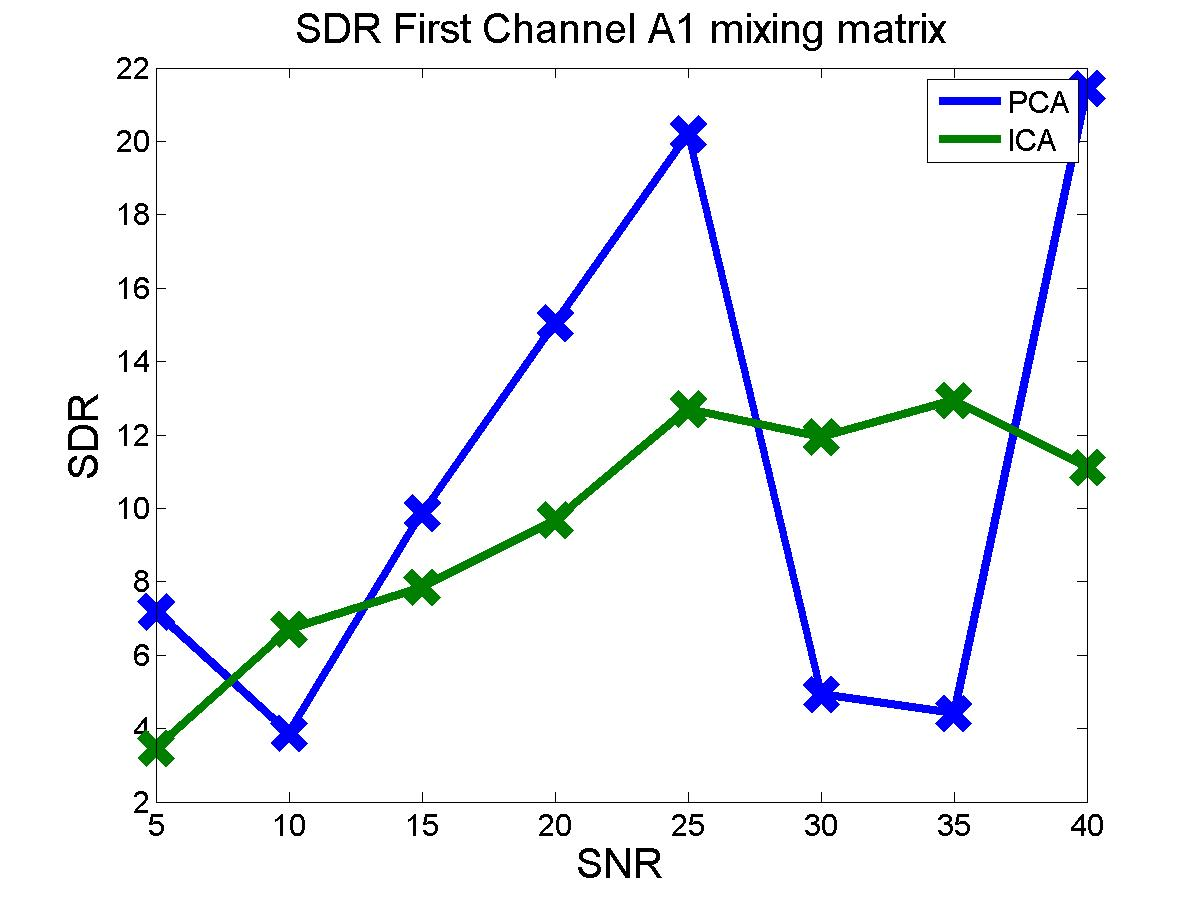
\includegraphics[width=.6\textwidth]{1.jpg}\\
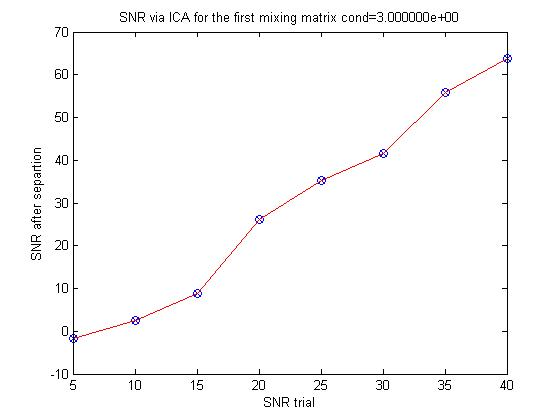
\includegraphics[width=.6\textwidth]{SNR1.jpg}\\
\tiny{First mixing matrix}\label{a1}
\endminipage\hfill
\minipage{.47\textwidth}%
\centering
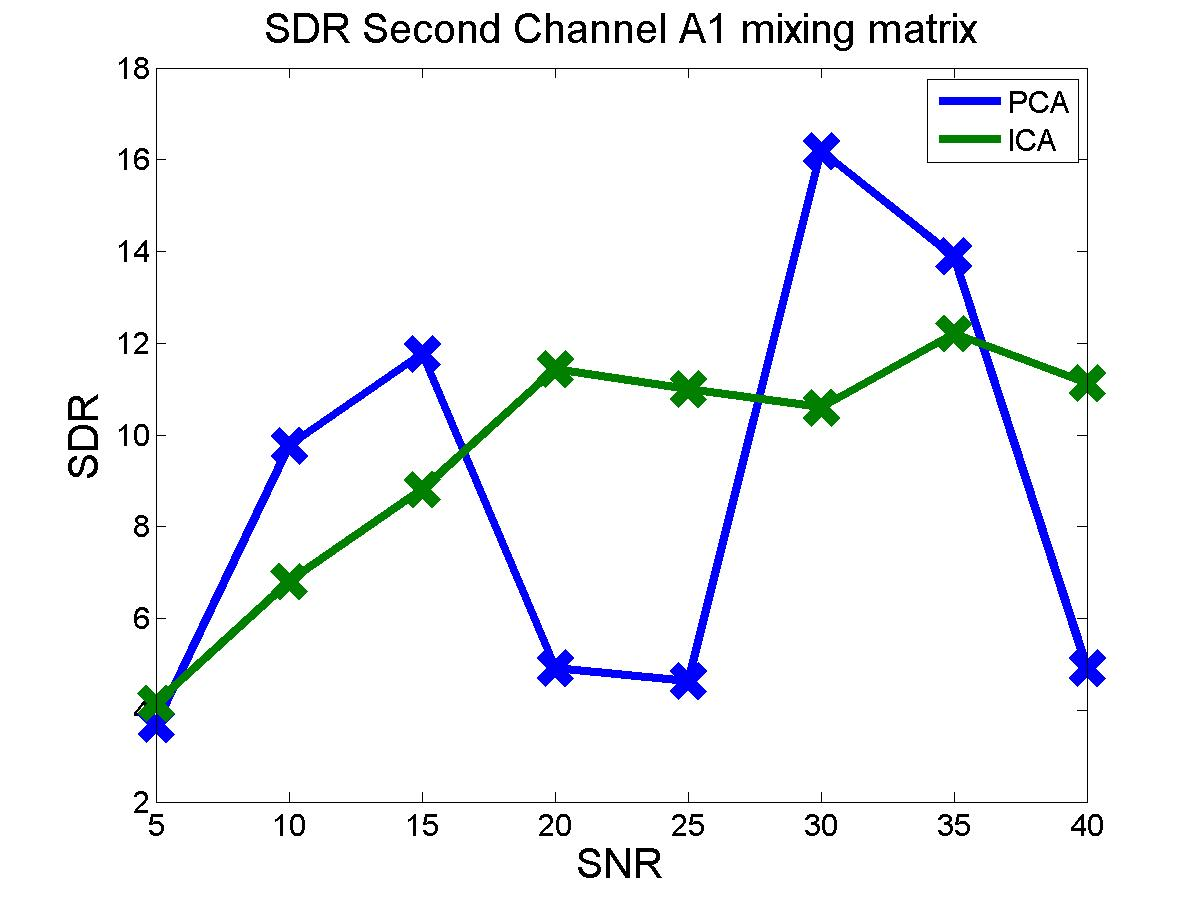
\includegraphics[width=.6\textwidth]{2.jpg}\\
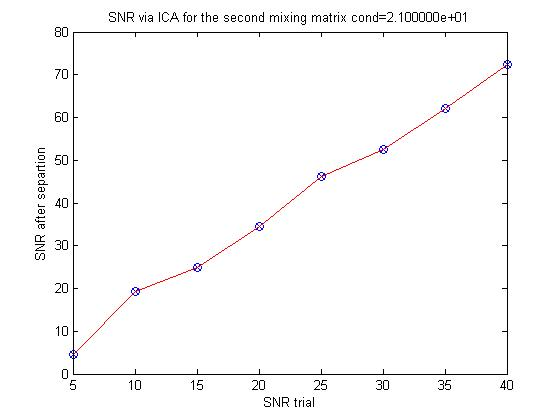
\includegraphics[width=.6\textwidth]{SNR2.jpg}\\
\tiny{Second mixing matrix}\label{a2}
\endminipage\hfill
\caption{\tiny Performance of ICA Implementation}
\end{figure}

\tiny{The 2-norm condition number for the first and the second matrix is fairly higher than on means both mixing matrices are just a bit far from the singularity where the mixing matrices are:\\
A1=[1 -2;-2 1];\\
A2=[1 -1.1;-1.1 1];}

\end{frame}

\begin{frame}{PCA implementation}

\begin{figure}[!htbp]
\minipage{.47\textwidth}%
\centering
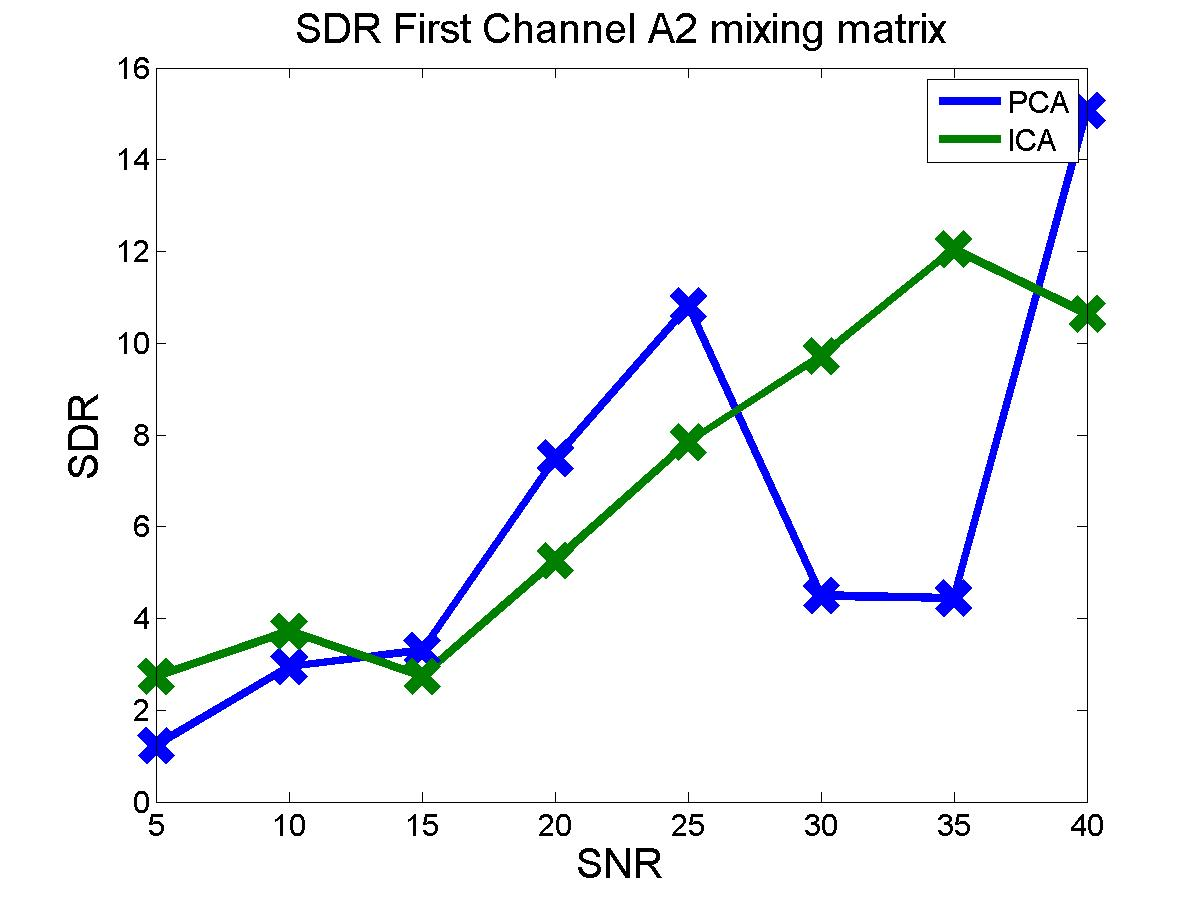
\includegraphics[width=.6\textwidth]{3.jpg}\\
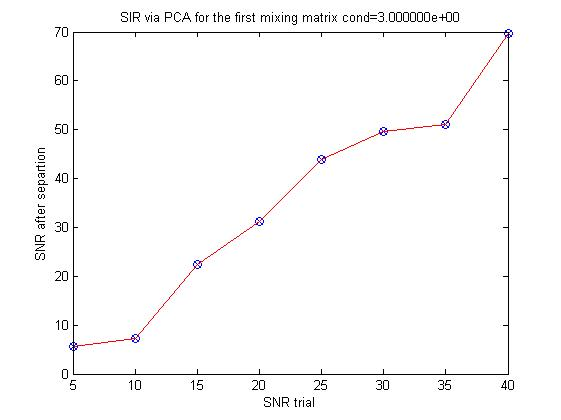
\includegraphics[width=.6\textwidth]{SNR3.jpg}\\
\tiny{First mixing matrix}\label{a3}
\endminipage\hfill
\minipage{.47\textwidth}%
\centering
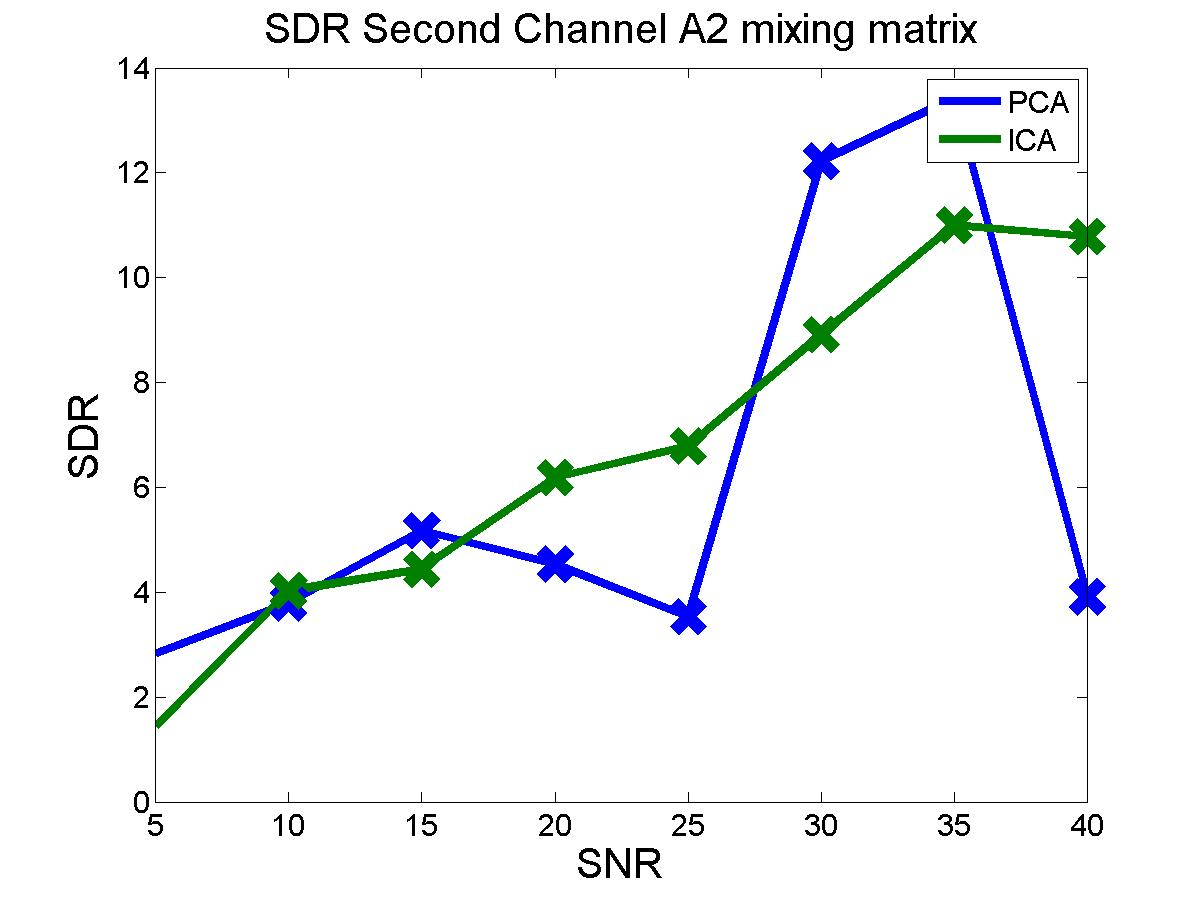
\includegraphics[width=.6\textwidth]{4.jpg}\\
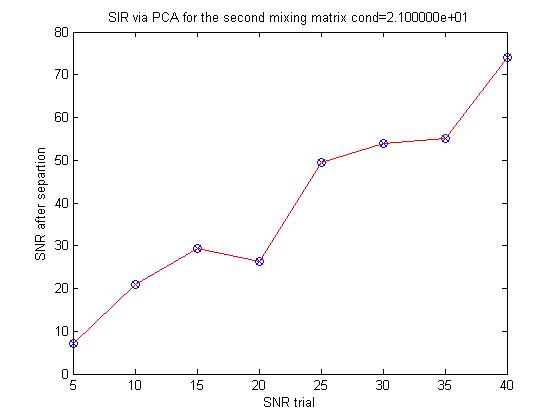
\includegraphics[width=.6\textwidth]{SNR4.jpg}\\
\tiny{Second mixing matrix}\label{a4}
\endminipage\hfill
\tiny {Performance of PCA Implementation}
\end{figure}

\tiny{$[U1,Sing1,V1]=svd(M1,'econ');$\\
    $[U2,Sing2,V2]=svd(M2,'econ');$\\
    
    
    $x1^{est}_{PCA}=V1(:,1:2)';$\\
    $x2^{est}_{PCA}=V2(:,1:2)';$\\
    
    $A1_{h}_{PCA}=M1*pinv(x1^{est}_{PCA});$\\
    $A2_{h}_{PCA}=M2*pinv(x2^{est}_{PCA});$\\}
    
 
\end{frame}

\section{FEGG data}
\begin{frame}{COM2}

\begin{figure}[!htbp]
\minipage{.47\textwidth}%
\centering
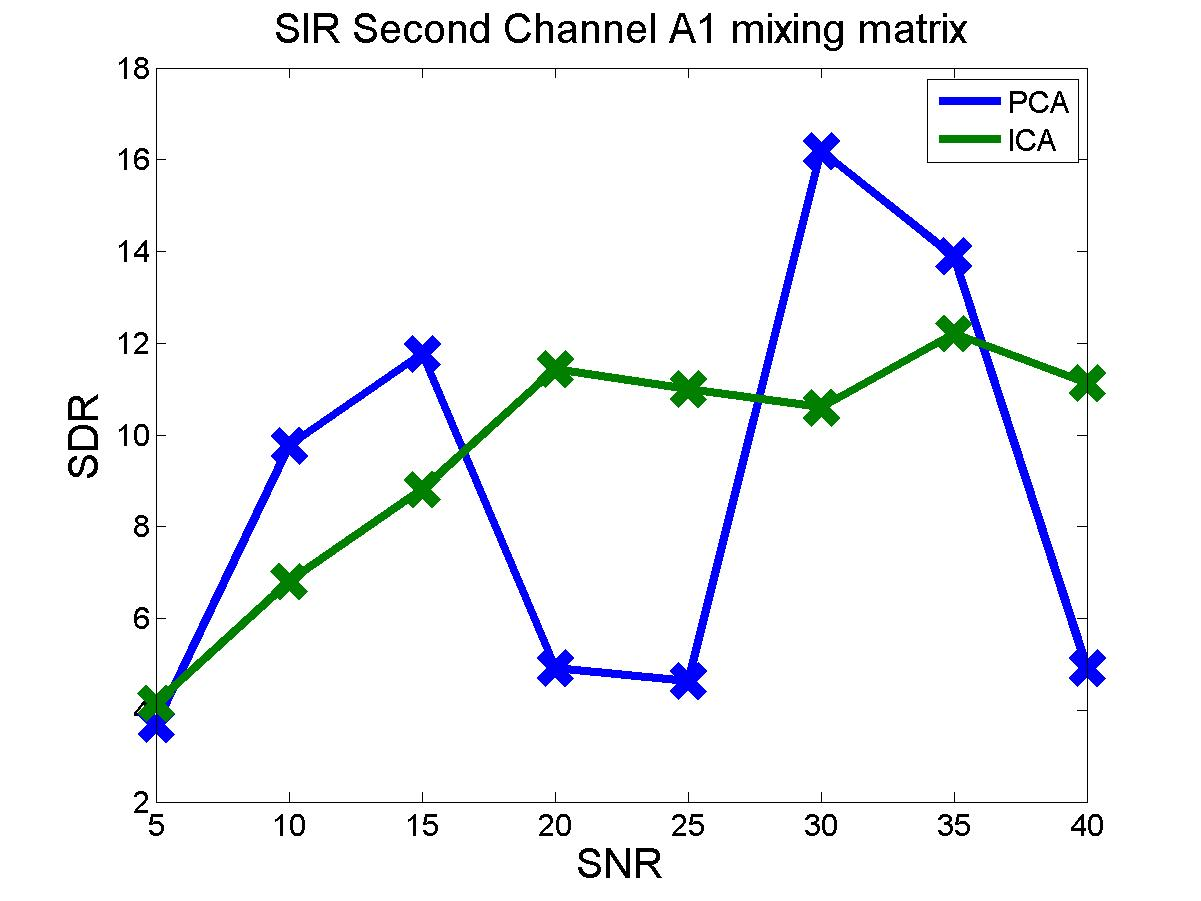
\includegraphics[width=1\textwidth]{6.jpg}\\
\tiny{Channel data before ICA}\label{a9}
\endminipage\hfill
\minipage{.47\textwidth}%
\centering
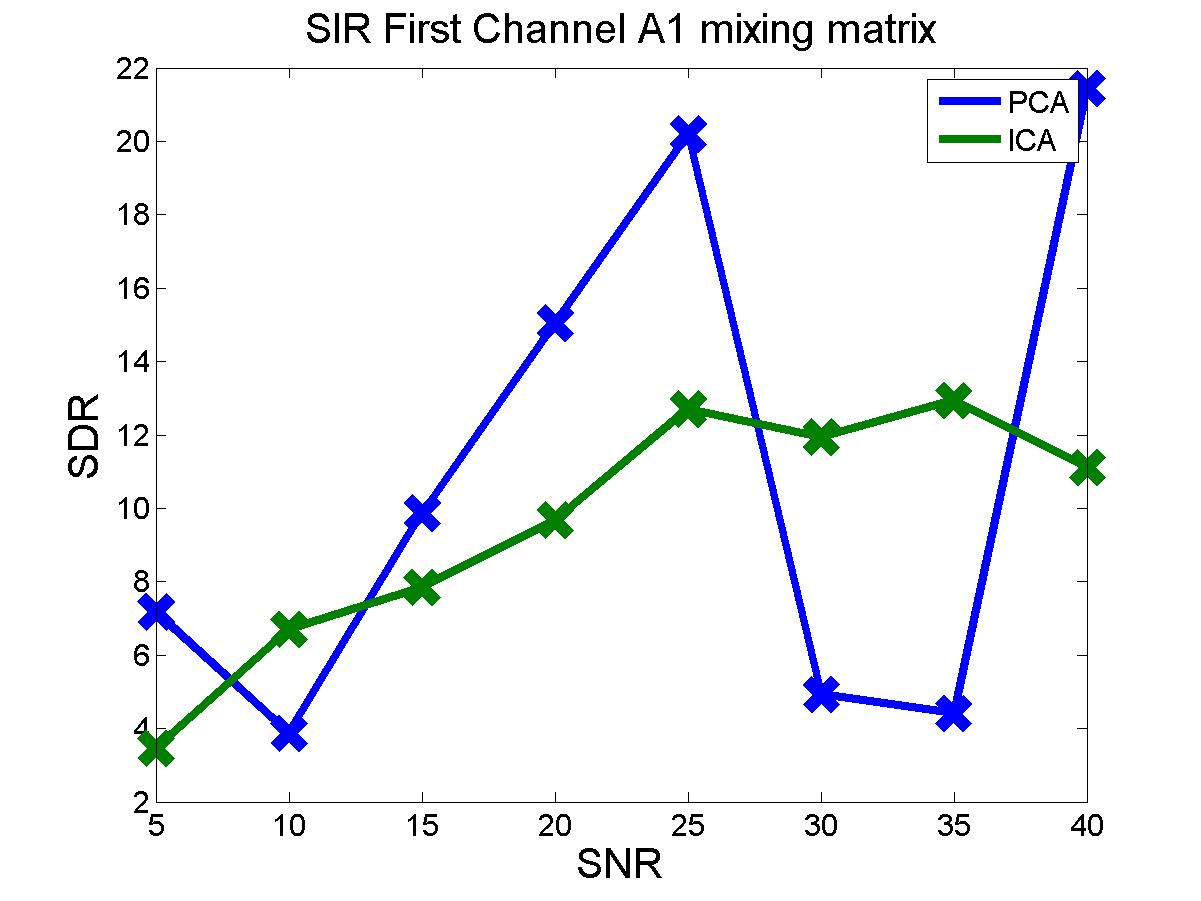
\includegraphics[width=1\textwidth]{5.jpg}\\
\tiny{Channel after before ICA}\label{a10}
\endminipage\hfill
\caption{\tiny ICA separation via COM2 method}
\end{figure}
  
\end{frame}


\section{Synthetic CP data}

\begin{frame}{CPD}
\begin{figure}[!htbp]
\minipage{.3\textwidth}%
\centering
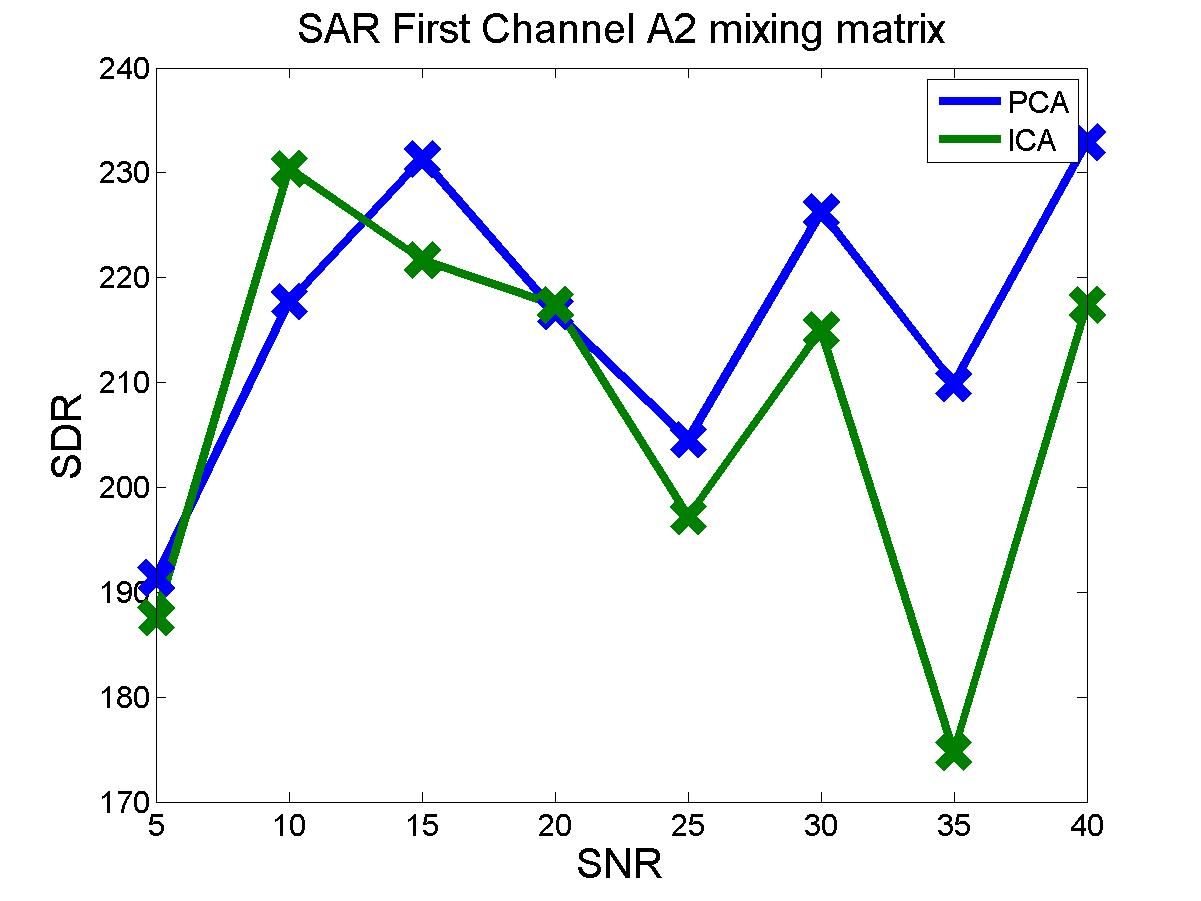
\includegraphics[width=1\textwidth]{11.jpg}\\
\tiny{A}
\endminipage\hfill
\minipage{.3\textwidth}%
\centering
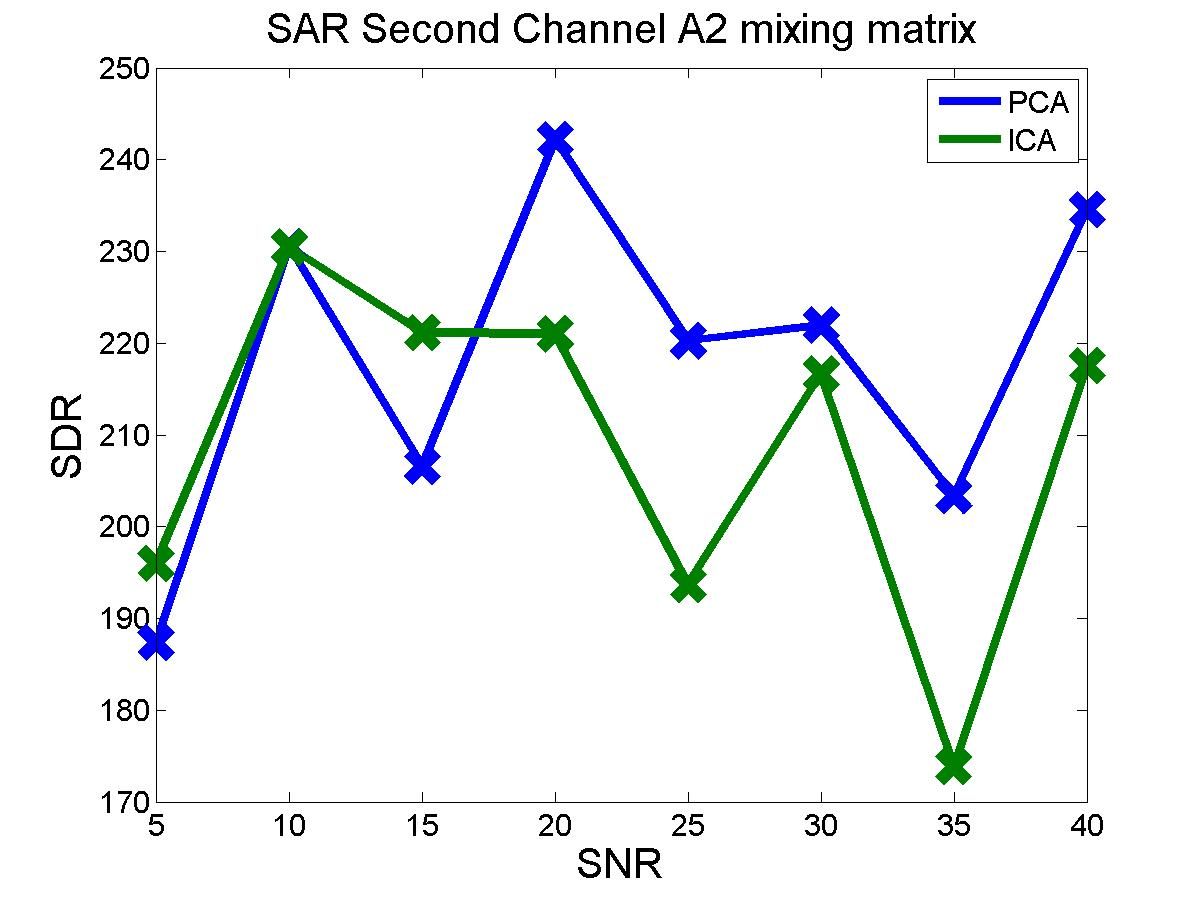
\includegraphics[width=1\textwidth]{12.jpg}\\
\tiny{B}
\endminipage\hfill
\minipage{.3\textwidth}%
\centering
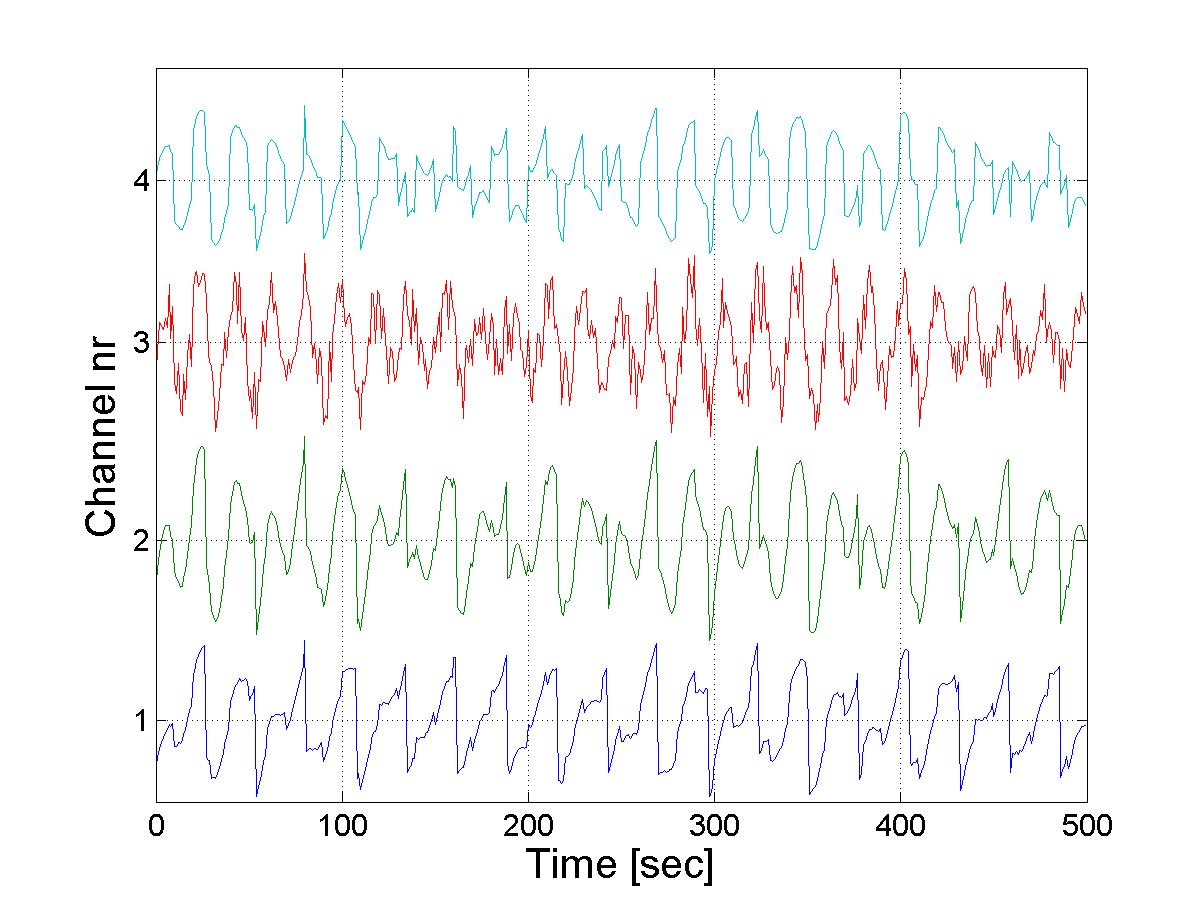
\includegraphics[width=1\textwidth]{13.jpg}\\
\tiny{C}
\endminipage\hfill
\caption{\tiny CPD components}\label{a15}
\end{figure}

\begin{equation}
    T=\sum_{r=1}^{3}a_{r}\#b_{r}\#c_{r}
\end{equation}

\end{frame}

\begin{frame}{SVD}

 \begin{figure}[!htbp]
\minipage{.3\textwidth}%
\centering
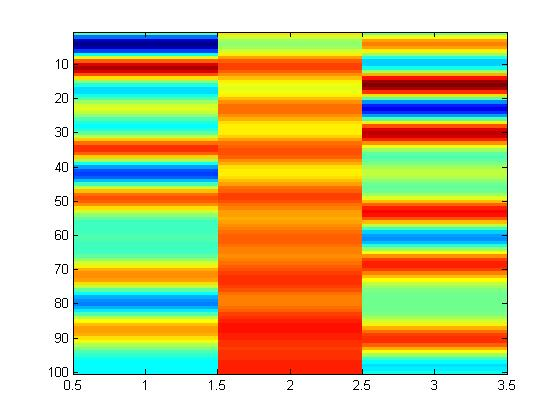
\includegraphics[width=1\textwidth]{26.jpg}\\
\tiny{A}
\endminipage\hfill
\minipage{.3\textwidth}%
\centering
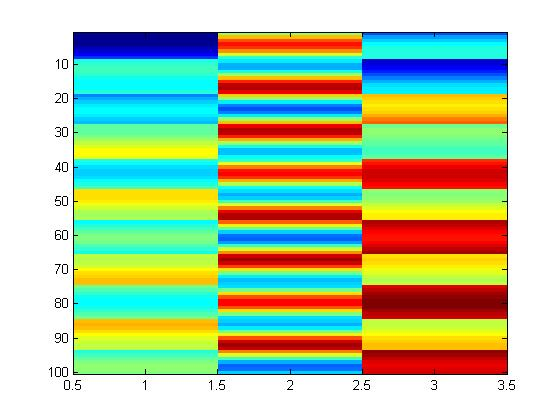
\includegraphics[width=1\textwidth]{25.jpg}\\
\tiny{B}
\endminipage\hfill
\minipage{.3\textwidth}%
\centering
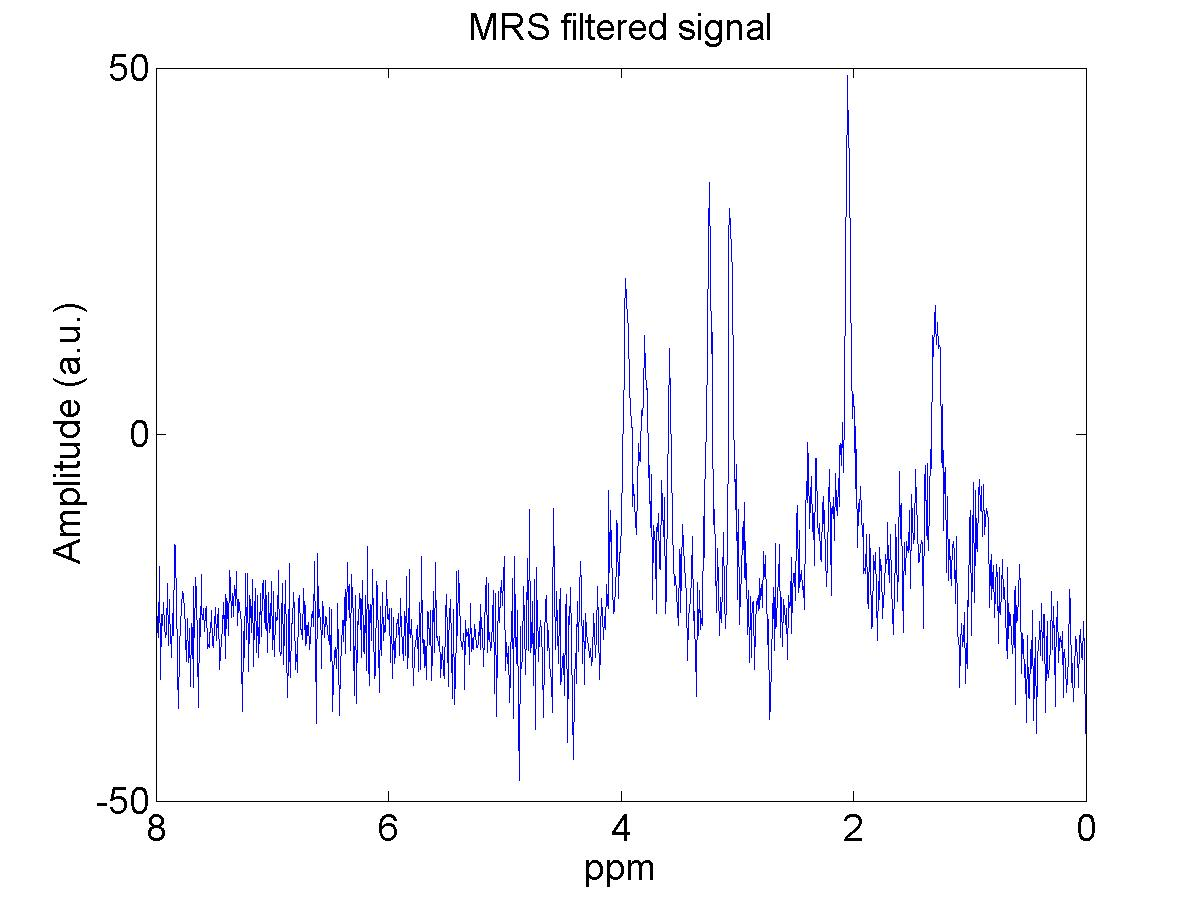
\includegraphics[width=1\textwidth]{24.jpg}\\
\tiny{C}
\endminipage\hfill
\caption{\tiny Components via SVD}\label{A1}
\end{figure}

\end{frame}



\begin{frame}{Iterative rank estimation}

\begin{figure}[!htbp]
\minipage{.47\textwidth}%
\centering
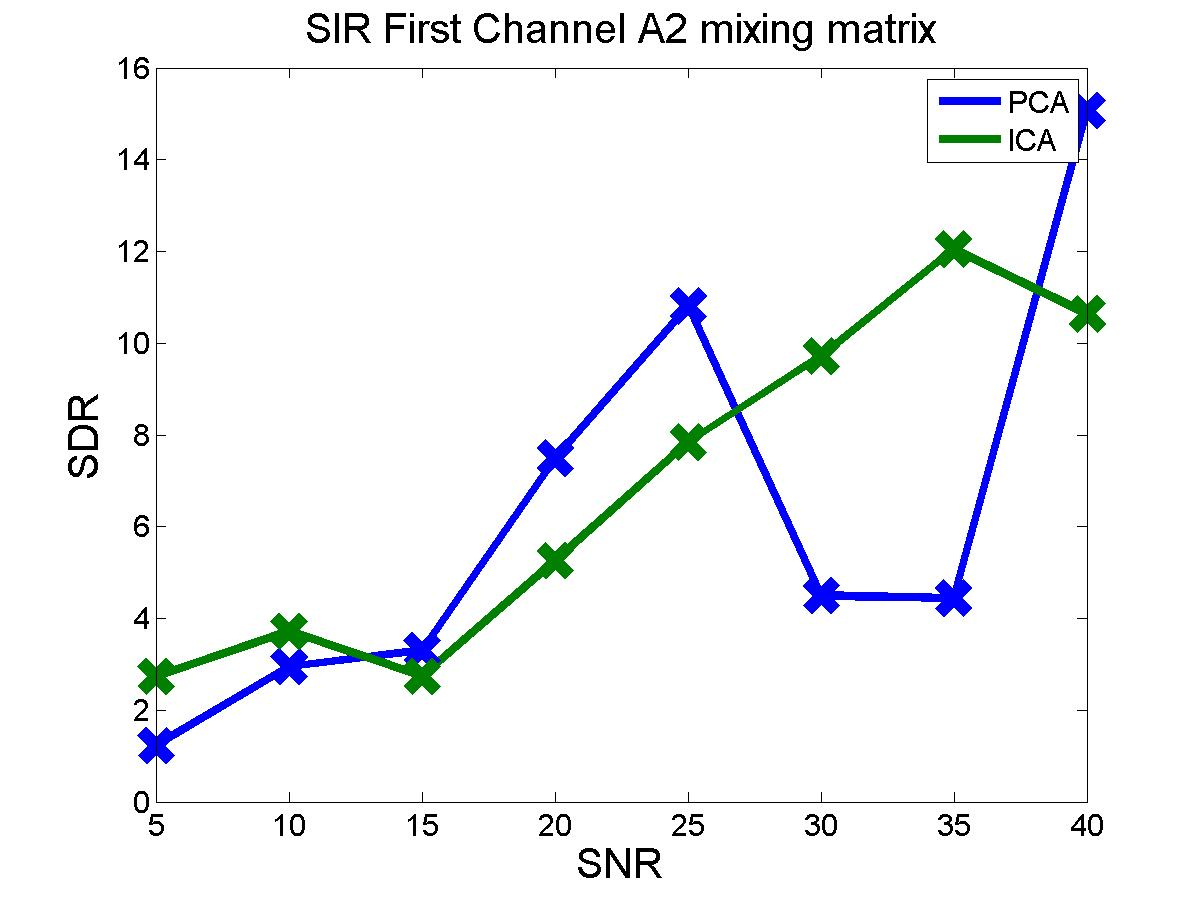
\includegraphics[width=1\textwidth]{7.jpg}\\
\tiny{Freb norm over different iteration}\label{a13}
\endminipage\hfill
\minipage{.47\textwidth}%
\centering
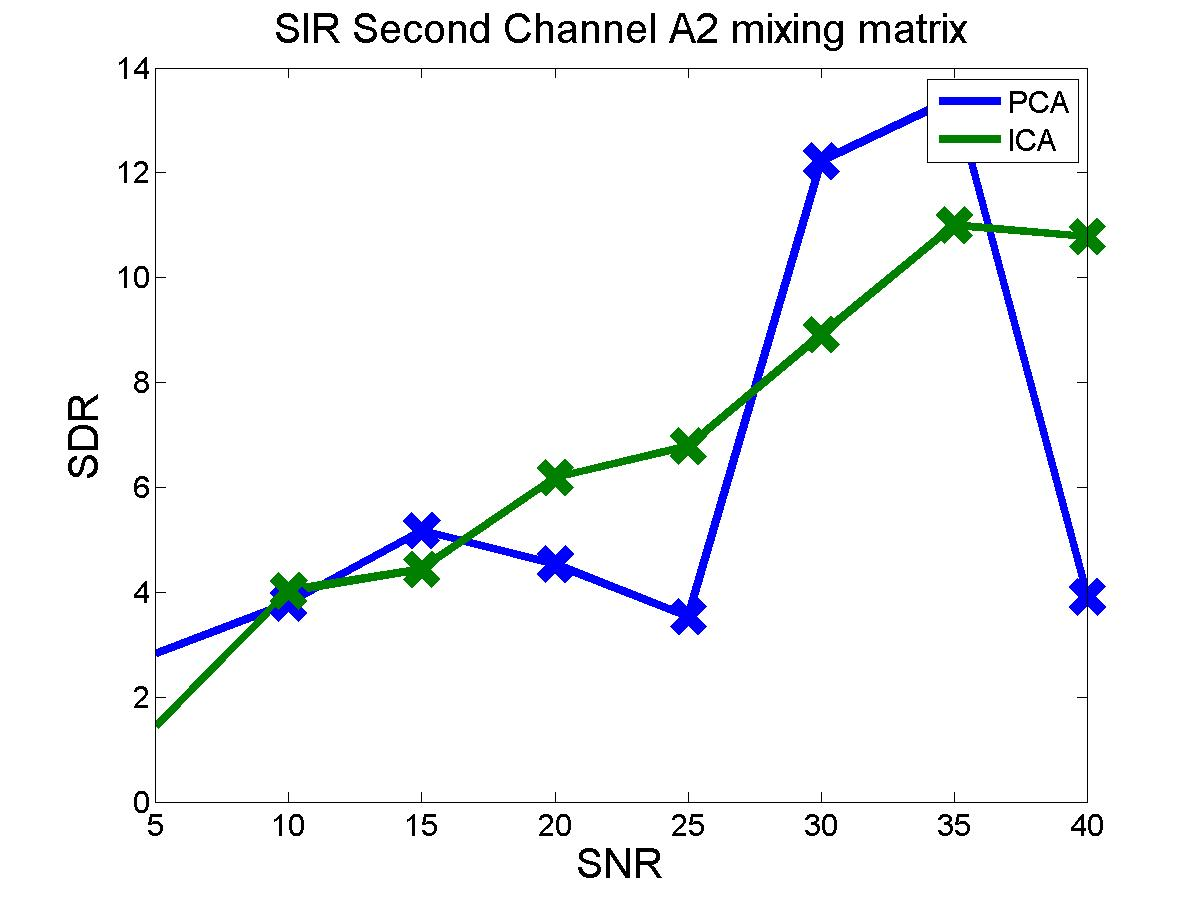
\includegraphics[width=1\textwidth]{8.jpg}\\
\tiny{Relative error of estimation}\label{a14}
\endminipage\hfill
\end{figure}


\end{frame}





\begin{frame}{Multilinar SVD}

\begin{figure}[!htbp]
\minipage{.47\textwidth}%
\centering
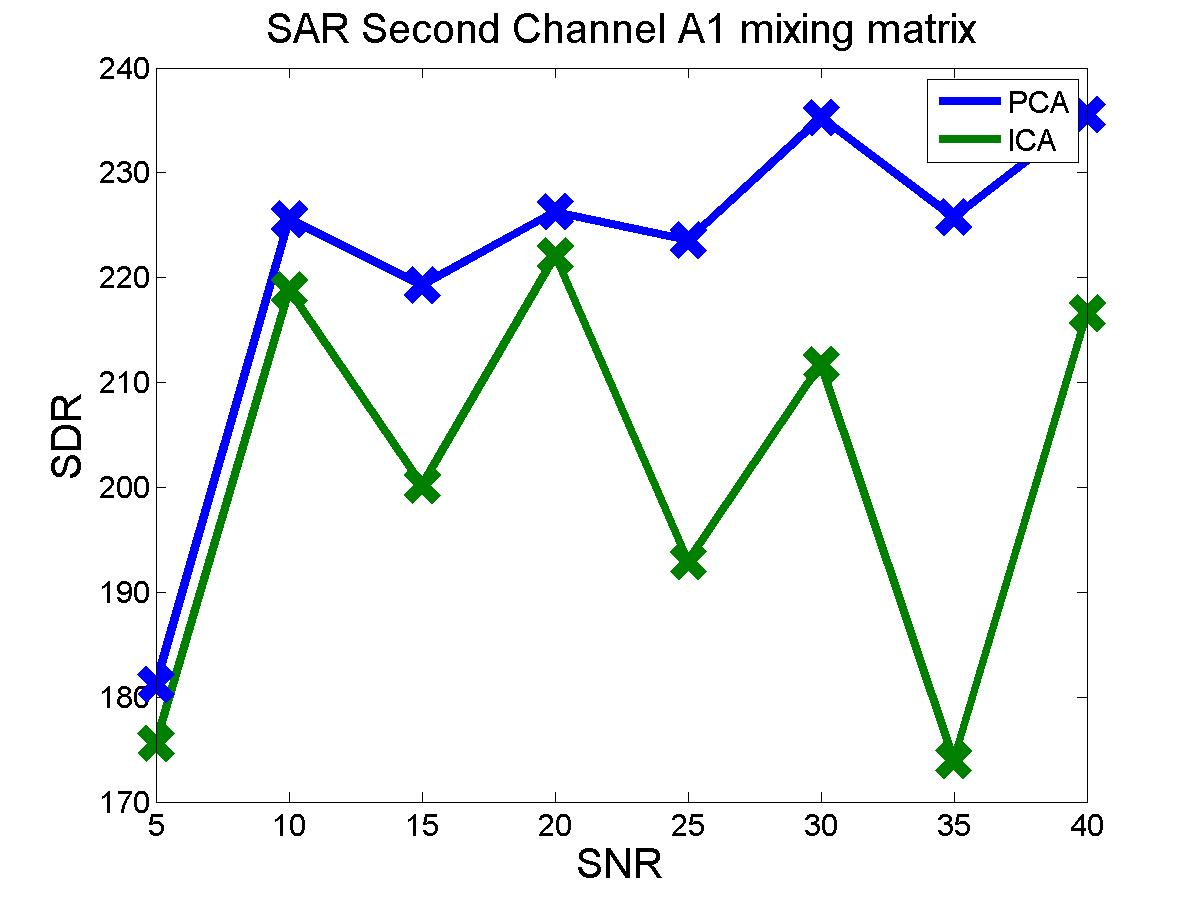
\includegraphics[width=1\textwidth]{10.jpg}\\
\tiny{Multilinear singular values in the noisy case}\label{a11}
\endminipage\hfill
\minipage{.47\textwidth}%
\centering
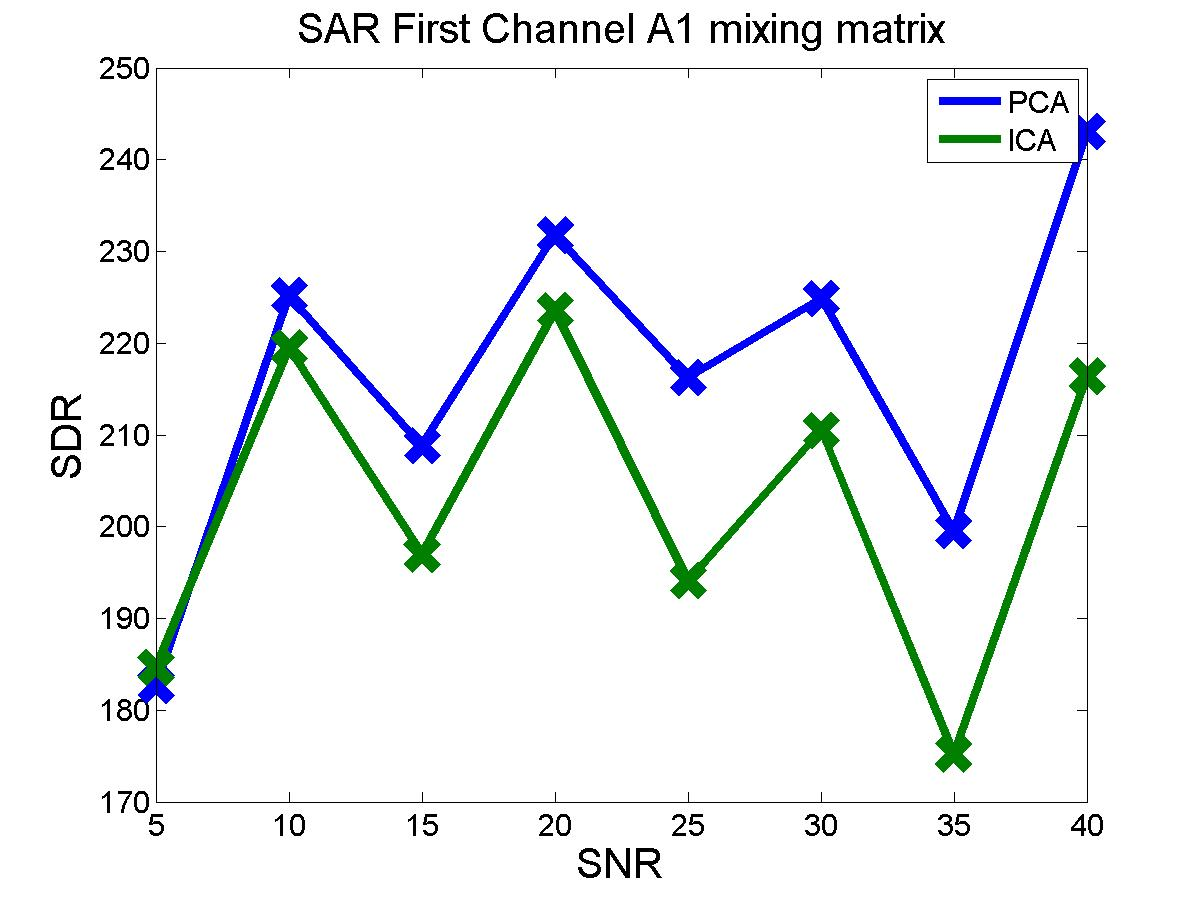
\includegraphics[width=1\textwidth]{9.jpg}\\
\tiny{Multilinear singular values in the noiseless case}\label{a12}
\endminipage\hfill
\caption{\tiny Multilinear singular values}
\end{figure}


\end{frame}



\section{Epilepsy data}

\begin{frame}{Tensorization of the EEG signals}

\begin{figure}[!htbp]
\minipage{.3\textwidth}%
\centering
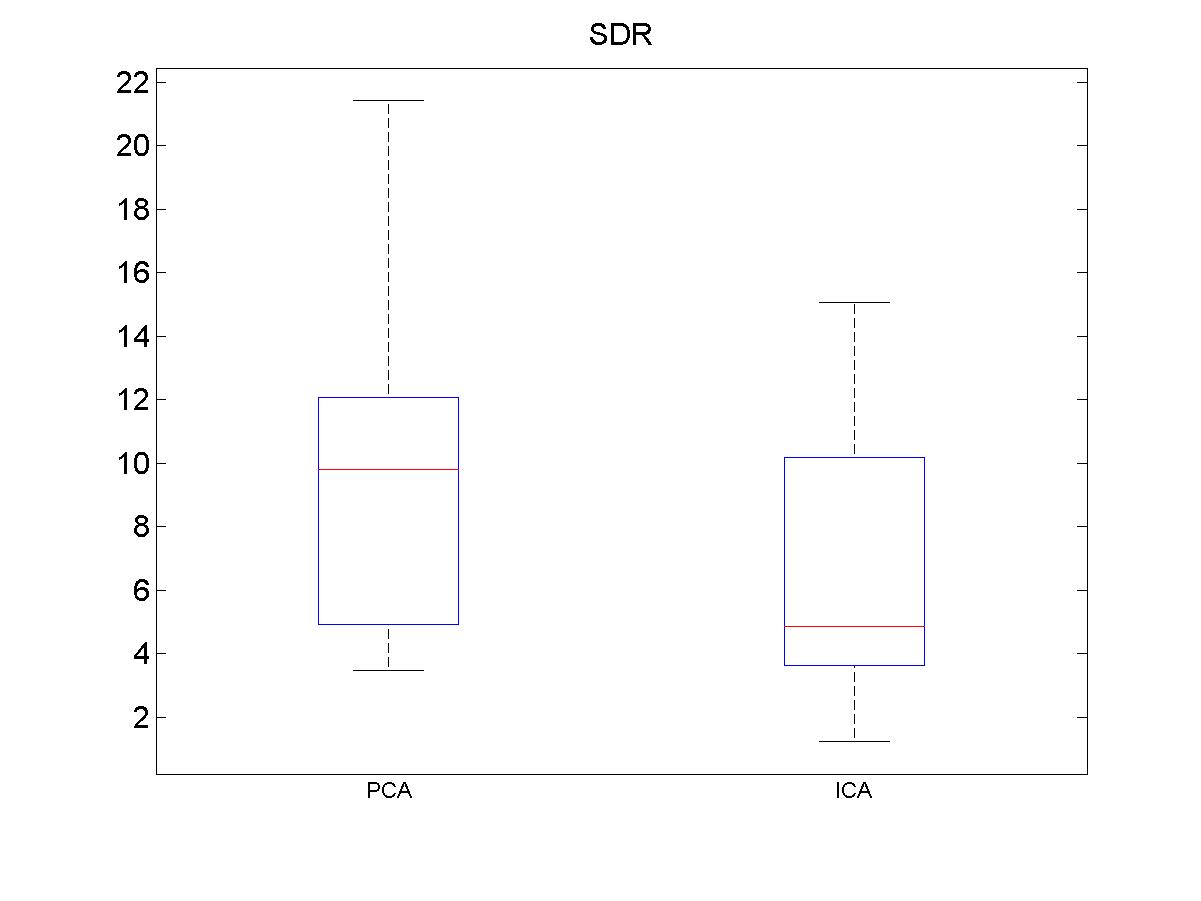
\includegraphics[width=1\textwidth]{15.jpg}
\endminipage\hfill
\minipage{.3\textwidth}%
\centering
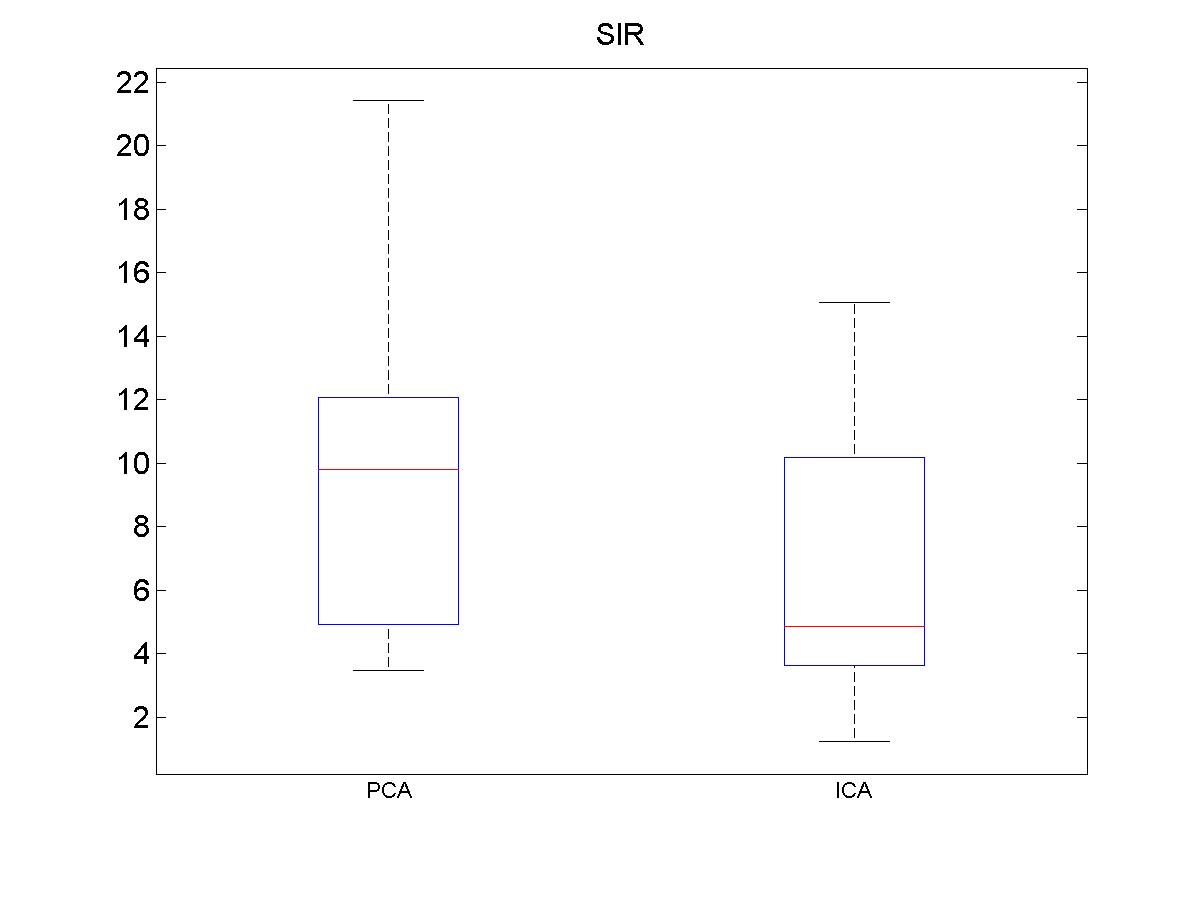
\includegraphics[width=1\textwidth]{16.jpg}
\endminipage\hfill
\minipage{.3\textwidth}%
\centering
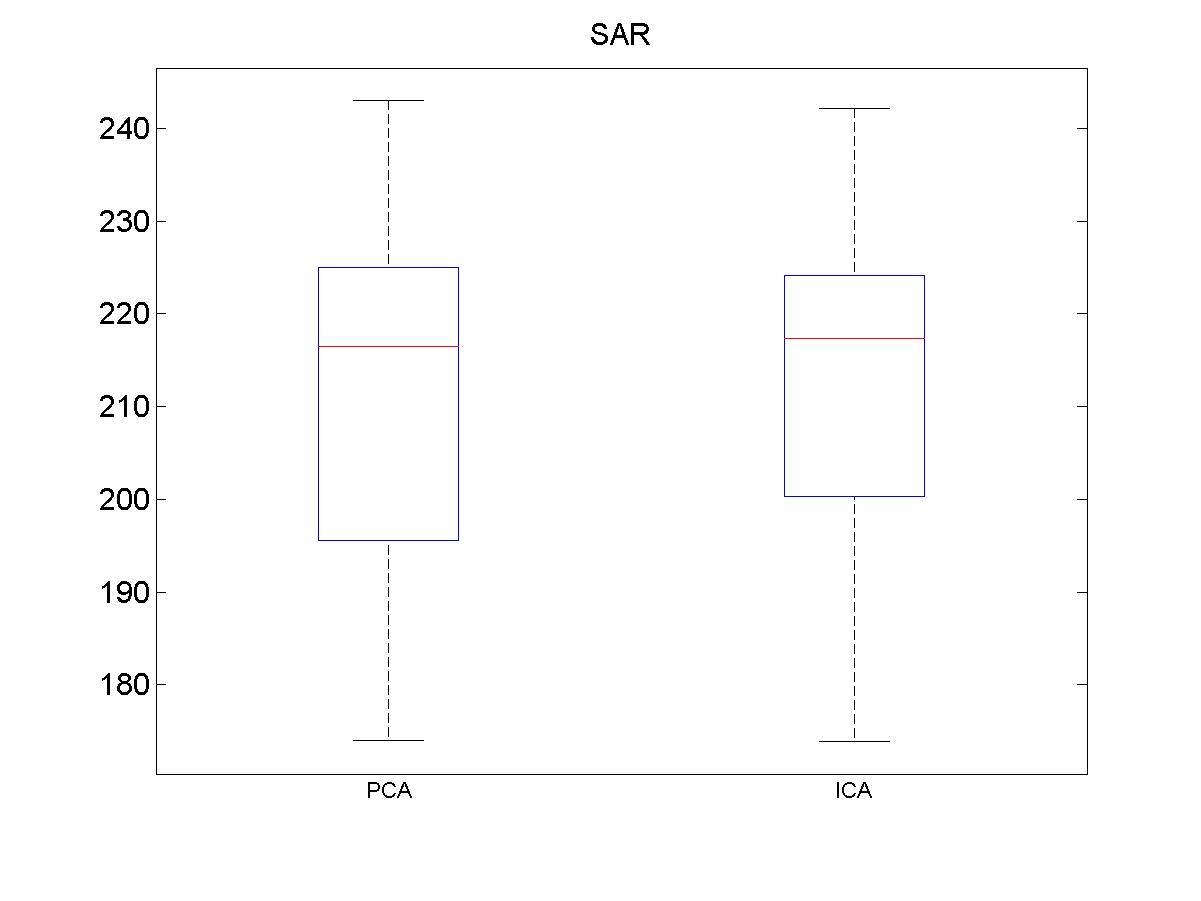
\includegraphics[width=1\textwidth]{17.jpg}
\endminipage\hfill
\end{figure}

\begin{figure}[!htbp]
\centering
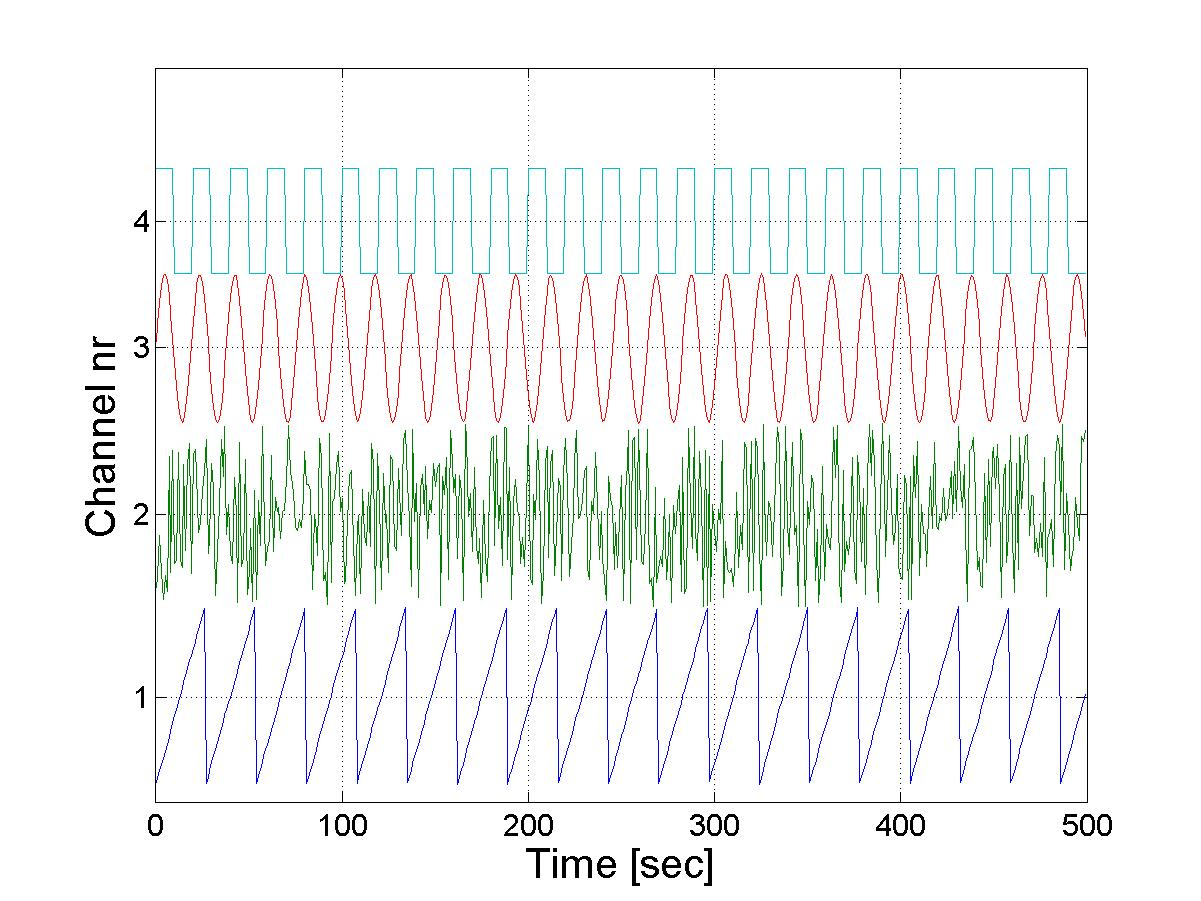
\includegraphics[width=.4\textwidth]{14.jpg}\\
\tiny {Channel data}\label{a17}
\end{figure}

\end{frame}



\begin{frame}{Parameter estimation}
 
 \begin{figure}[!htbp]
\minipage{.47\textwidth}%
\centering
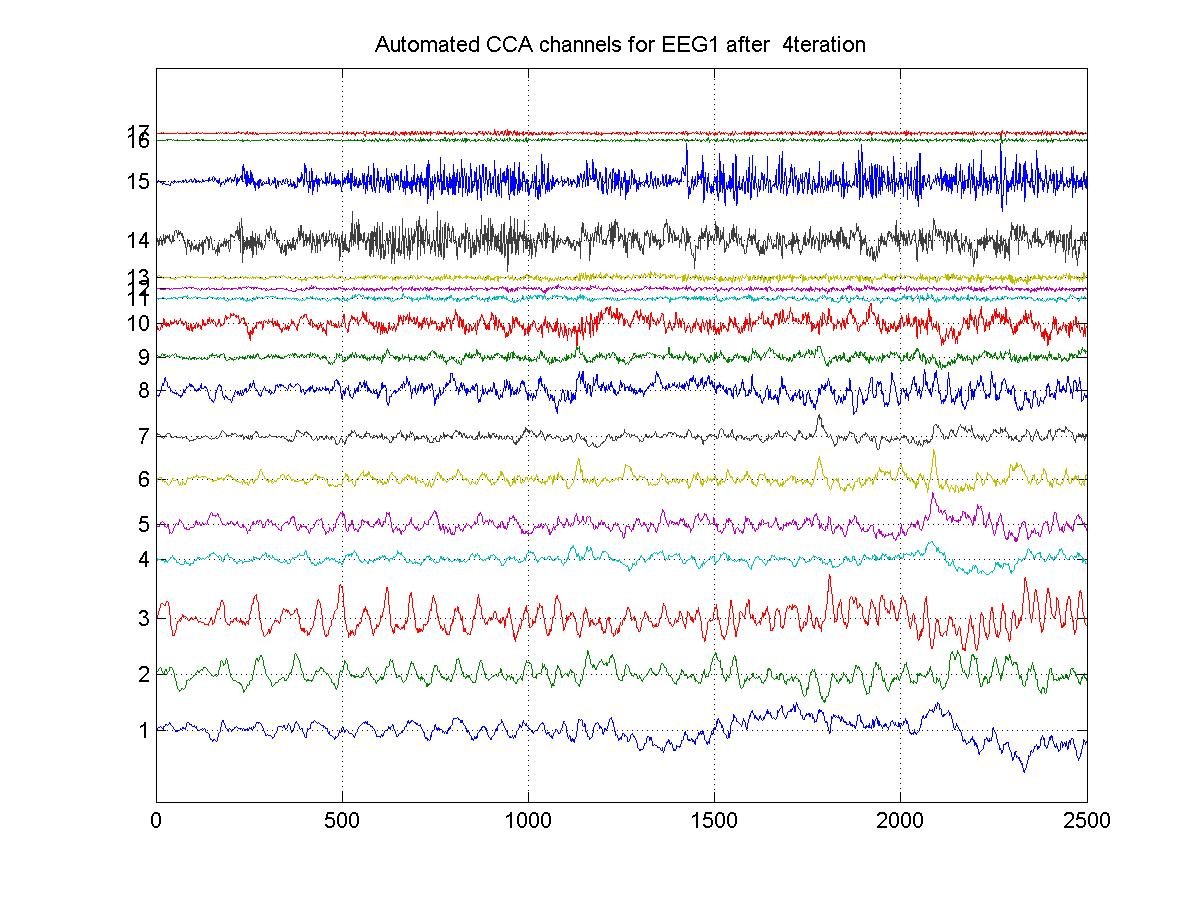
\includegraphics[width=1\textwidth]{18.jpg}\\
\tiny{Time resoltution}\label{a18}
\endminipage\hfill
\minipage{.47\textwidth}%
\centering
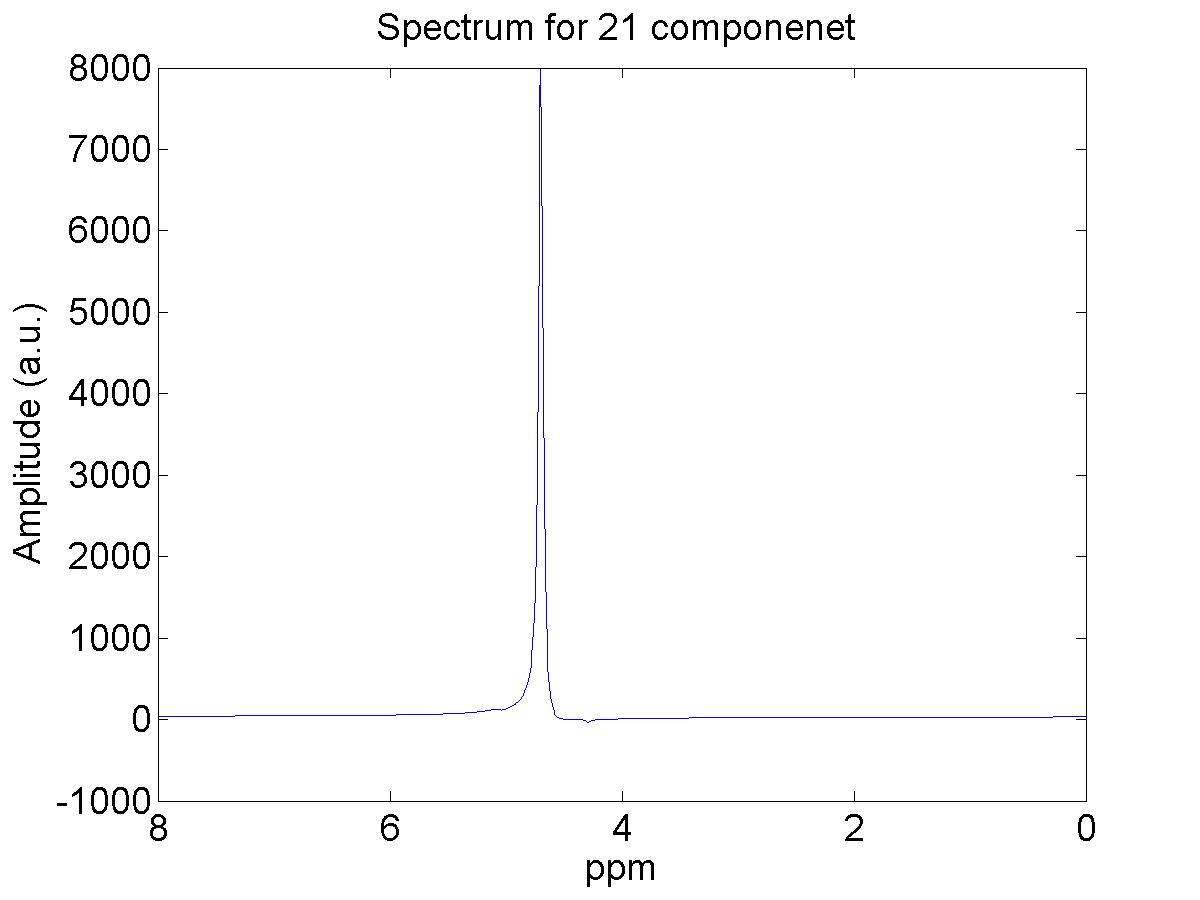
\includegraphics[width=1\textwidth]{19.jpg}\\
\tiny{Frequency resolution}\label{a19}
\endminipage\hfill
\end{figure}

\end{frame}



\begin{frame}{Voltage profile for the normal brain activity }

\begin{figure}[!htbp]
\minipage{.4\textwidth}%
\centering
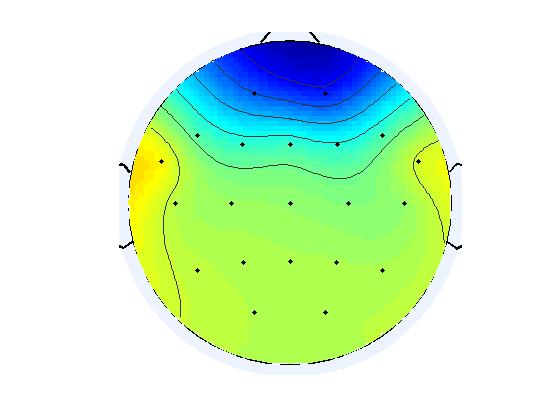
\includegraphics[width=1\textwidth]{20.jpg}\\
\tiny{Normal event}\label{a20}
\endminipage\hfill
\minipage{.4\textwidth}%
\centering
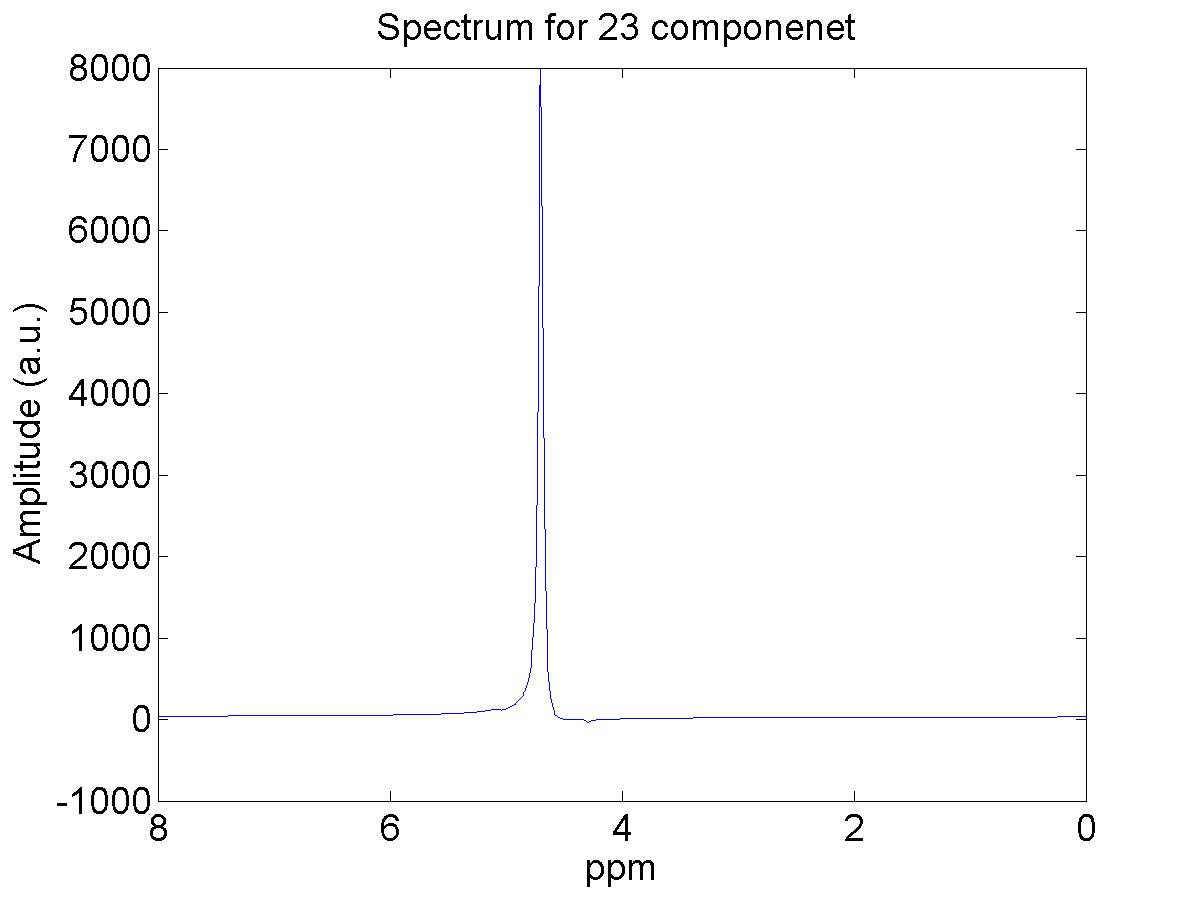
\includegraphics[width=1\textwidth]{21.jpg}\\
\tiny{Epilepsy}\label{a21}
\endminipage\hfill
\minipage{.4\textwidth}%
\centering
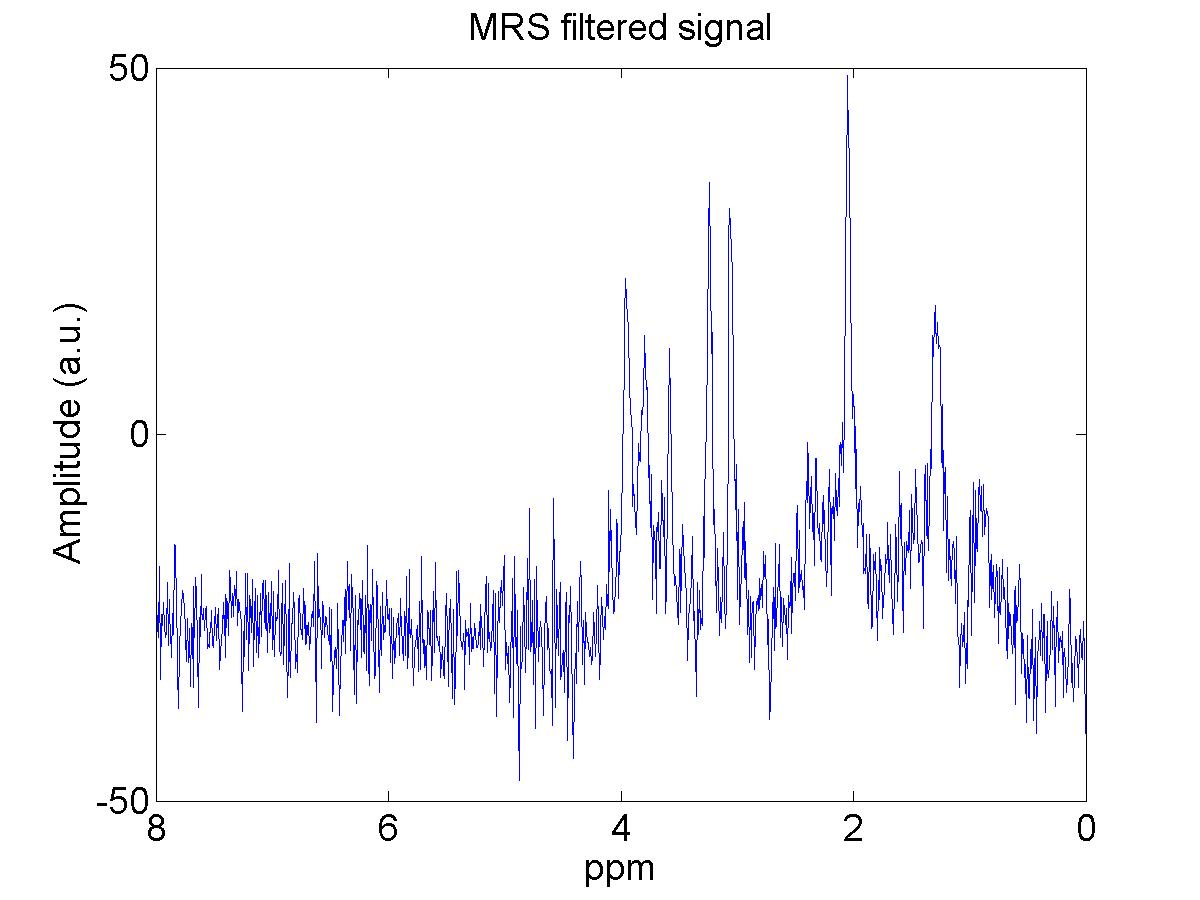
\includegraphics[width=1\textwidth]{22.jpg}\\
\tiny{Epilepsy}\label{a22}
\endminipage\hfill
\minipage{.4\textwidth}%
\centering
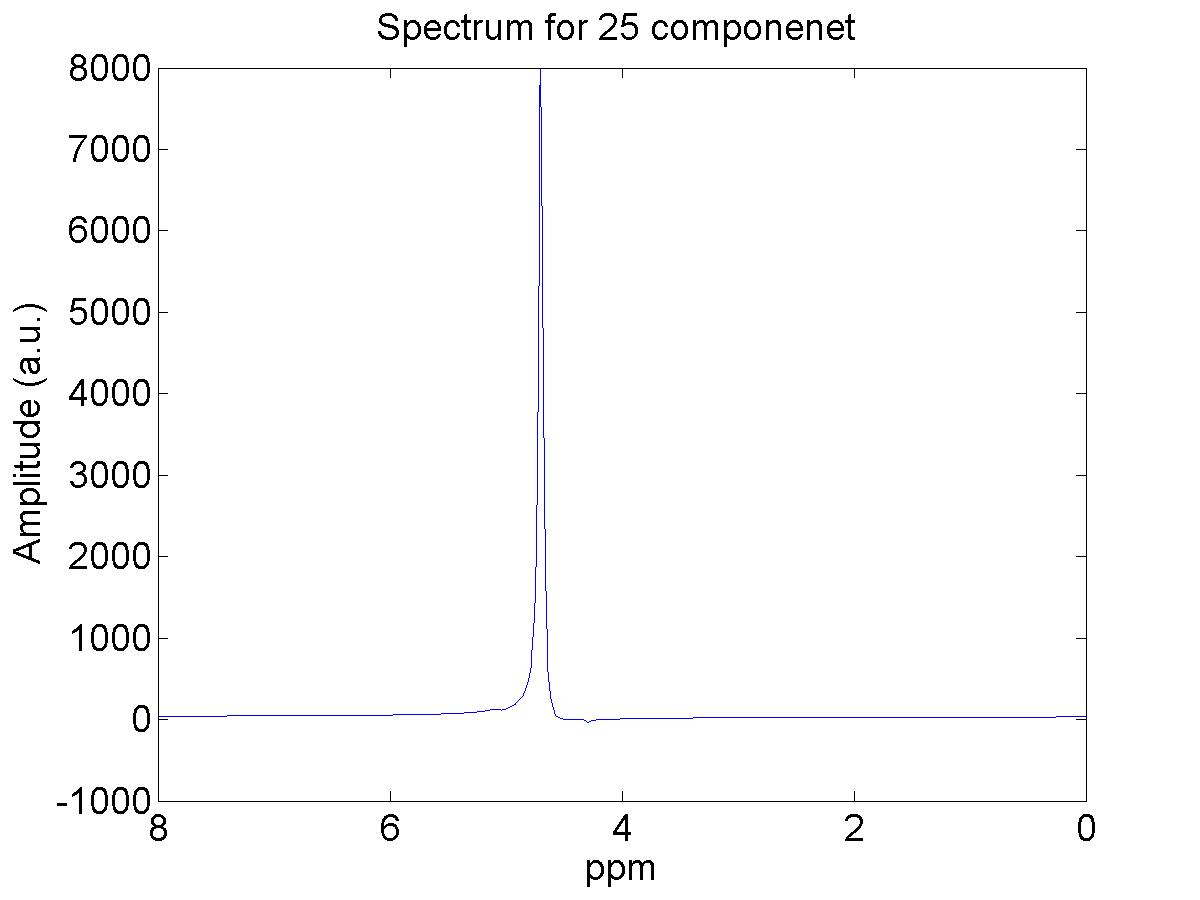
\includegraphics[width=1\textwidth]{23.jpg}\\
\tiny{Epilepsy}\label{a23}
\endminipage\hfill
\end{figure}

\end{frame}

\begin{frame}{Iterative rank estimation}
\begin{figure}[!htbp]
\centering
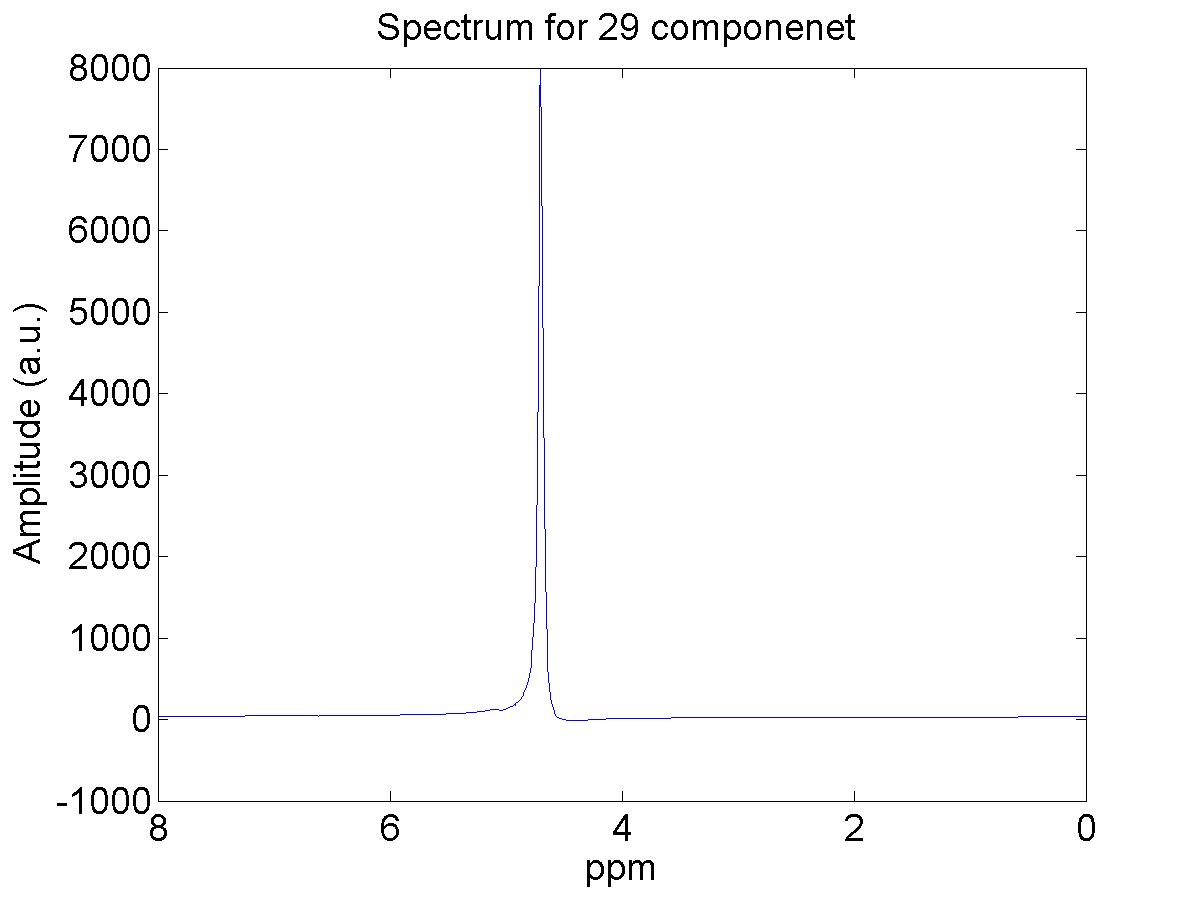
\includegraphics[width=.6\textwidth]{27.jpg}
\caption{Rank estimation}\label{A2}

\end{figure}   
\end{frame}


\emptyfooter
\begin{frame}{ }
\centering \textbf{\Large \textit{Thank you for your attention!}}
\begin{figure}[!htb]

\includegraphics[width=.3\textwidth]{QA.jpg}
\end{figure}
\largefooter
\end{frame}






\end{document}